\documentclass[12pt,a4paper]{report}
					
					\usepackage[titles]{tocloft}
					\newlength{\mylen} % a scratch length
					\renewcommand{\cftfigpresnum}{Gambar } % goes before figure number
					\settowidth{\mylen}{\cftfigpresnum} % space required to print \cftfigpresnum
					\addtolength{\mylen}{\cftfignumwidth} % plus space for the number
					\setlength{\cftfignumwidth}{1cm} % but make this zero
					\renewcommand{\cftfigaftersnumb}{\hspace{\mylen}} % add space after the zero-spaced number
					\renewcommand{\cfttabpresnum}{Tabel } % repeat above for Tables
					\settowidth{\mylen}{\cfttabpresnum}
					\addtolength{\mylen}{\cfttabnumwidth}
					\setlength{\cfttabnumwidth}{1 em}
					\renewcommand{\cfttabaftersnumb}{\hspace{\mylen}}
					 \renewcommand \cftchapdotsep{4.5}

\renewcommand{\baselinestretch}{2.0}			%Mengubah spasi menjadi 1.5
\renewcommand{\chaptername}{\large{BAB }}		%Mengubah kata menjadi Bab
\renewcommand{\figurename}{\textbf{Gambar}}		%Mengubah kata menjadi Gambar
\renewcommand{\contentsname}{DAFTAR ISI}		%Mengubah kata menjadi Daftar Isi
\renewcommand{\listfigurename}{DAFTAR GAMBAR}	%Mengubah kata menjadi Daftar Gambar
\renewcommand{\listtablename}{DAFTAR TABEL}		%Mengubah kata menjadi Daftar Tabel
\renewcommand{\tablename}{\textbf{Tabel}}		%Mengubah kata menjadi Tabel
\renewcommand\bibname{DAFTAR PUSTAKA}			%Mengubah kata menjadi Referensi
%\newcommand{\keyword}{\textit{keyword}}
\usepackage[left=4cm,top=4cm,right=3cm,bottom=3cm]{geometry}
\usepackage[font = small]{caption}
\usepackage{booktabs}
\usepackage{graphicx}			%Library untuk gambar
\usepackage{fancyhdr}			%Library untuk menggunakan header
\usepackage{caption}			%Library untuk mengubah caption
%\usepackage{subcaption}			%Library untuk mengubah subcaption
\usepackage{subfig}				%Library untuk membuat subfigure (gambar yang berseblahan dan berurutan)
\usepackage{tocbibind}			%Library untuk menambahkan daftar isi, gambar, dan tabel ke table of contents
\usepackage{parskip}			%Library untuk menghapus paragraf indent
\setlength{\parskip}{1em}		%Add space between paragraph
\usepackage{enumitem}			%Library edit enumerate dan itemize
\usepackage{titlesec}			%Library edit title spacing
\usepackage{sectsty}
\usepackage{multirow}
\usepackage{array}
\usepackage{booktabs}
\usepackage{mathtools}
\usepackage{amssymb, amsmath} 	% needed for math
\usepackage{siunitx}
\usepackage{url}
\usepackage{hyperref}
\usepackage[backend=bibtex,style=numeric,sorting=none]{biblatex}
\usepackage{listings}
\usepackage{array}
\newcolumntype{P}[1]{>{\centering\arraybackslash}p{#1}}

\usepackage{indentfirst}
\setlength{\parindent}{0.5cm}
\usepackage[utf8]{inputenc}
%\usepackage{fontspec}
\usepackage{setspace}
\usepackage{siunitx}
\usepackage{pslatex}
\usepackage{chngcntr}
\counterwithin*{equation}{chapter}
\usepackage{multicol}
\usepackage{upgreek}
\newcommand{\bra}[1]{\ensuremath{\left\langle#1\right|}}
\newcommand{\ket}[1]{\ensuremath{\left|#1\right\rangle}}

%\setmainfont{Times New Roman}
\lstset{
numbers=left, 
numberstyle=\small, 
numbersep=3pt, 
  basicstyle=\small,
  columns=fullflexible,
  frame=tb,
  breaklines=true,
  framexleftmargin=1pt,
  tabsize=1
}
\addbibresource{referensi.bib}
\fancypagestyle{plain}{
  	\fancyhf{}% Clear header/footer
    \fancyfoot[R]{\thepage}% Right footer
}
\fancypagestyle{awalbab}{
  \renewcommand{\headrulewidth}{0pt}% Remove header rule
  \renewcommand{\footrulewidth}{0pt}% Remove footer rule
  \fancyhf{}% Clear header/footer
  \fancyfoot[C]{A-\thepage}
}

\fancypagestyle{myplain}
{
  \fancyhf{}
  \renewcommand\headrulewidth{0pt}
  \renewcommand\footrulewidth{0pt}
  \fancyfoot[C]{\thepage}
}

\pagestyle{plain}
\lhead{}
\chead{}
\rhead{\thepage}
\cfoot{}
\lfoot{}
\rfoot{}
\renewcommand{\headrule}{}
\renewcommand{\headrulewidth}{0pt}
\renewcommand{\footrulewidth}{0pt}
%\bibliographystyle{unsrt}
\bibliography{dapus,up,cite_gambar}
%================Mengubah ukuran font pada section, subsection, dll================
\sectionfont{\normalsize}
\subsectionfont{\normalsize}
\titleformat{\section}{\large\bfseries}{\thesection}{1em}{}
\titlespacing\section{0pt}{12pt plus 4pt minus 2pt}{0pt plus 2pt minus 2pt}
\titlespacing\subsection{0pt}{12pt plus 4pt minus 2pt}{0pt plus 2pt minus 2pt}
\titlespacing\subsubsection{0pt}{12pt plus 4pt minus 2pt}{0pt plus 2pt minus 2pt}
%========================Mengubah spacing pada awal chapter========================
\titleformat{\chapter}[display]
	{\normalfont\large\bfseries\centering}{\chaptertitlename \thechapter \centering}{-10pt}{\large}
\titlespacing*{\chapter}{0pt}{-30pt}{20pt}
%==================================================================================
\tolerance=1
\emergencystretch=\maxdimen
\hyphenpenalty=10000
\hbadness=10000

\begin{document}
	\begin{onehalfspacing}
\begin{titlepage}
	\centering
	{\textbf{KALKULASI NILAI EIGEN BERBASIS MATRIKS HAMILTONIAN MENGGUNAKAN TEKNIK \textit{BLOCK MATRIX}: STUDI KASUS PADA \textit{GRAPHENE}}}

	\vspace{2cm}

	\textbf{SKRIPSI} \\
	\vspace{0.5cm}
	Diajukan sebagai Salah Satu Syarat untuk Menempuh Ujian Akhir Tingkat Sarjana pada Program Studi Fisika Fakultas Matematika dan Ilmu Pengetahuan Alam Universitas Padjadjaran

	\vspace{1cm}
	\textbf{Oleh: \\
	Mirza Aditya Deliantama\\
	140310170044}

	\vspace{1cm}
	\begin{figure}[!htbp]
		\centering
		
\includegraphics[width=3.5cm]{gambar/unpadbw.png}
		\label{cover}
	\end{figure}

	\vspace{3cm}
	{\textbf{PROGRAM STUDI FISIKA \\
	FAKULTAS MATEMATIKA \& ILMU PENGETAHUAN ALAM \\
	UNIVERSITAS PADJAJARAN \\
	2021 \\}}
\end{titlepage}

\setcounter{page}{2}
\pagenumbering{roman}
%\chapter*{\centering ABSTRAK}

%\addcontentsline{toc}{chapter}{ABSTRAK}

%\chapter*{\centering ABSTRACT}

%\addcontentsline{toc}{chapter}{ABSTRACT}

\chapter*{\centering LEMBAR PENGESAHAN}
\thispagestyle{empty}
\begin{tabular}{p{3cm}p{11cm}}
JUDUL \hspace{1.4cm}:&  KALKULASI NILAI EIGEN BERBASIS MATRIKS HAMILTONIAN MENGGUNAKAN TEKNIK \textit{BLOCK MATRIX} : STUDI KASUS PADA \textit{GRAPHENE} \\
PENYUSUN \hspace{0.5cm}:&  MIRZA ADITYA DELIANTAMA \\
NPM \hspace{1.83cm}:&  140310170044 \\
LAB \hspace{1.89cm}:&  FISIKA INSTRUMENTASI \\
\end{tabular}
\vspace{1cm}
\begin{center}
Jatinangor, Juli 2021 \\
Menyetujui, \\
\begin{multicols}{2}
	{Pembimbing Utama \\
	\vspace{3cm}
	\underline{Prof. Dr. I Made Joni, M.Sc.} \\
	NIP. 19720601 200112 1 001 \\}

	{Pembimbing Pendamping \\
	\vspace{3cm}
	\underline{Dr. Ferry Faizal, Ph.D.} \\
	NIP. 19820531 201903 3 001\\}
\end{multicols}
\vspace{1cm}
Mengetahui, \\
Ketua Program Studi Fisika \\
Fakultas Matematika dan Ilmu Pengetahuan Alam \\
Universitas Padjadjaran \\
\vspace{3cm}
\underline{Dr. Andri Abdurrochman, S.Si, MT.} \\
NIP. 19740526 200312 1 002 \\

\end{center}
\end{onehalfspacing}
\addcontentsline{toc}{chapter}{LEMBAR PENGESAHAN}
\chapter*{\centering KATA PENGANTAR}
\thispagestyle{myplain}
 \hspace{5mm} 
 Dengan nama Allah yang Maha Pengasih dan Maha Penyayang. Alhamdulillaahirabbil'aalamiin, segala puji hanya milik Allah 'azza wa jalla karena berkat-Nya skripsi yang berjudul "Kalkulasi nilai eigen berbasis matriks Hamiltonian menggunakan Teknik \textit{Block Matrix} : studi kasus pada \textit{Graphene}" sebagai salah satu syarat menyelesaikan pendidikan tingkat sarjana pada Program Studi Fisika, Fakultas Matematika dan Ilmu Pengetahuan Alam, Universitas Padjadjaran dapat selesai. Tak lupa terimakasih kepada Drs. Enung Achmad S., M.Pd., dan Lilis Susilayati, S.H., yaitu orang tua penulis yang selalu memberi dukungan kepada penulis sehingga penulis dapat menyelesaikan dengan sebaik mungkin. Penulis juga mengucapkan terimakasih kepada pihak-pihak yang membantu penulis untuk menyelesaikan tugas akhir ini:
\begin{enumerate}
	\item Dekan Fakultas Matematika dan Ilmu Pengetahuan Alam Universitas Padjadjaran, Prof. Dr. Iman Rahayu, M.Sc.
	\item Kepala Departemen Fisika FMIPA Unpad, Prof. Dr. Camellia Panatarani
	\item Ketua Program Studi Fisika FMIPA Unpad, Dr. Andri Abdurrochman, S.Si, MT.
	\item Prof. Dr. Eng. I Made Joni, M.Sc., selaku pembimbing utama dan dosen wali yang telah yang selalu memberikan bimbingan, dukungan, bantuan secara materi dan psikis dan fasilitas terbaik kepada penulis selama penelitian dan kuliah
	\item Prof. Dr. Eng Camellia Panatarani, M.Si., yang selalu memberikan ilmu, dukungan dan fasilitas terbaik kepada penulis selama menyelesaikan skripsi
	\item Ferry Faizal, Ph.D., selaku pembimbing pendamping yang selalu memberikan bimbingan, saran dan masukan, bantuan, dukungan, fasilitas dan arahan terbaiknya kepada penulis
	\item Dr. Wildan Abdussalam, yang selalu memberikan bimbingan, motivasi, bantuan, dan arahan yang membuat penulis selalu bersemangat saat menyelesaikan skripsi
	\item Pa Setianto, Pa Ocik, Kang Dwindra, dan seluruh civitas FiNder-U CoE yang membantu penulis menyelesaikan skripsi
	\item Nurfauzi Fadillah yang telah memberikan bantuan, dukungan, fasilitas dan motivasi kepada penulis
	\item P-Labs sebagai tempat penulis untuk membuat, merevisi dan menyelesaikan skripsi dengan menyenangkan
	\item Ferdian, Syakir, Yoga, Felix, Hilmy, Ahmad, Victor, Naufal, Ghemma, Fahmi, Bayu, Reyhan, Budi, dan Urfan yang telah memberikan kebahagiaan, dukungan dan bantuan kepada penulis selama menyelesaikan skripsi
	\item Revani dan Fahriza yang telah memberikan dukungan dan bantuan saat mengadakan pemaparan kemajuan mingguan agar skripsi ini dapat selesai dengan baik
	\item Lutfi Naufal Ramadhika dan Lucia Patia Rochman yang telah memberikan dukungan moril kepada penulis saat menyelesaikan skripsi
	\item Atom 2017 yang telah mewarnai masa kuliah penulis
	\item Tim KBK Instrumentasi dan Elektronika yang selalu membuat penulis bersemangat untuk mengerjakan skripsi
\end{enumerate}

Dengan segala kerendahan hati, penulis menyadari bahwa skripsi ini masih memiliki banyak kekurangan dan jauh dari kesempurnaan. Oleh karena itu, kritik dan saran yang membangun sangat dibutuhkan oleh penulis. Semoga skripsi ini dapat bermanfaat bagi perkembangan ilmu dan teknologi serta bagi pihak-pihak yang membutuhkan.
\vspace{2cm}
\begin{flushright}
	Jatinangor, Juli 2021\\
	\vspace{2cm}
	Penulis
\end{flushright}
\addcontentsline{toc}{chapter}{KATA PENGANTAR}


\chapter*{\centering ABSTRAK}
\thispagestyle{myplain}
\begin{spacing}{1.0}
\noindent Senyawa kimia organik adalah salah satu senyawa kimia yg sering diteliti, salah satu cara untuk meneliti senyawa tersebut adalah dengan menggunakan pendekatan kuantum yg disebut Kimia Fisik. Graphene merupakan salah satu senyawa kimia organik yang dapat diamati karakteristiknya dengan menggunakan Teori Hückel, yang akan melihat interaksi antar ikatan-$\pi$ dalam senyawa tersebut. Penggunaan kalkulasi eigen dari persamaan Schrödinger tak bergantung waktu akan menghasilkan nilai energi orbital molekul dan nilai konstanta gelombang. Kedua nilai inilah yang akan digunakan untuk mencari nilai absorbsi. Ketika menggunakan matriks Hamiltonian yang ukurannya besar, maka akan menyebabkan adanya \textit{bottleneck} dalam memproses data. Agar performa komputasinya tidak menurun, digunakan perhitungan menggunakan teknik \textit{Block Matrix} dan teknik \textit{Big Data}. Hasil penelitian menunjukkan bahwa, semakin banyak atom karbon yang dimiliki Graphene akan membuat celah energi yang dihasilkan semakin kecil yang diakibatkan oleh menurunnya jarak antara energi orbital molekul. Selain itu dihasilkan juga performa komputasi tercepat untuk menghitung celah energi, yaitu dengan menggunakan PySpark. Nilai perubahan eksitasi energi dan momen dipol transisi yang didapatkan dari kalkulasi nilai eigen akan menggambarkan grafik absorpsi terhadap energi eksitasinya, dimana titik absorbsi tertinggi menggambarkan titik celah energinya.\\
\textbf{Kata kunci: \textit{Graphene, Teori Hückel, Teori Pita, Energi Absorbsi, PySpark}}
\end{spacing}
\addcontentsline{toc}{chapter}{ABSTRAK}

\chapter*{\centering \textit{ABSTRACT}}
\thispagestyle{myplain}
\begin{spacing}{1.0}
\noindent Organic chemical compounds are one of the chemical compounds that are often studied, one way to investigate these compounds is to use a quantum approach called Physycochemical. Graphene is one of the organic chemical compounds whose characteristics can be observed using the Hückel Theory, which will look at the interactions between $\pi$-bond in these compounds. The use of the eigen calculation of the time-independent Schrödinger equation will yield the energy values of the molecular orbitals and the value of the wave constant. These two values will be used to find the absorption value. When using a larger Hamiltonian matrix, it will cause a bottleneck in processing the data. So that the computational performance does not decrease, calculations using the Block Matrix technique and the Big Data technique are used. The results show that, the more carbon atoms that Graphene has, the smaller the energy gap produced due to the decrease in the distance between the molecular orbital energies. Moreover, the fastest computational performance for calculating the energy gap is also generated, namely by using PySpark. The value of the change in excitation energy and the transition dipole moment obtained from the calculation of the eigenvalues will describe the absorption graph of the excitation energy, where the highest absorption point describes the energy gap point.\\
\textbf{Keywords: \textit{Graphene, Hückel Theory, Band Theory, Absorbance Energy, PySpark}}
\end{spacing}
\addcontentsline{toc}{chapter}{ABSTRACT}

\thispagestyle{myplain}
\fancypagestyle{plain}{%
\fancyhf{}
\renewcommand{\headrulewidth}{0pt}
\fancyfoot[C]{\thepage}
}
\newpage
\normalsize {\tableofcontents}
\newpage
\normalsize {\listoffigures}
\newpage
\normalsize {\listoftables}

\renewcommand{\thechapter}{\Roman{chapter}}
\chapter*{BAB I \\ PENDAHULUAN}
\renewcommand{\thesection}{\arabic{section}}
\addcontentsline{toc}{chapter}{BAB I PENDAHULUAN}
\setcounter{chapter}{+1}
\thispagestyle{myplain}
\setcounter{page}{8}				%Mulai page numbering pada halaman 8
\pagenumbering{arabic}

\renewcommand{\thesection}{\arabic{chapter}.\arabic{section}}
\renewcommand{\thefigure}{\arabic{chapter}.\arabic{figure}}
\renewcommand{\thetable}{\arabic{chapter}.\arabic{table}}
\renewcommand{\theequation}{\arabic{chapter}.\arabic{equation}}
	\section{Latar Belakang}
	Kimia fisik adalah subdisiplin yang membahas tentang suatu kejadian physicochemical (fisiko-kimia) dengan menggunakan pendekatan secara atomik dan molekul dan benda terkondensasi dalam kacamata kefisikaan \cite{Slater1939}. Karena kimia fisik, maka akan sangat-sangat berkaitan dengan unsur yang ada di tabel periodik. Mulai dari unsur Hidrogen (H) dengan nomor atom 1, hingga unsur Oganeson (Og) dengan nomor atom 118. Salah satu bidang tentang kimia yaitu Kimia Organik. Kimia organik mempelajari tentang struktur, sifat, komposisi, reaksi, dan preparasi senyawa yang mengandung unsur karbon (C). Kimia organik tidak hanya mempelajari tentang hidrokarbon saja, namun ikatan antara karbon dengan senyawa lain seperti hidrogen, nitrogen, oksigen, sulfur, fosfor, silikon dan halogen \cite{ACS2020}. Salah satu senyawa kimia organik yang saat ini sedang diteliti yaitu graphene. Graphene merupakan salah satu senyawa kimia turunan dari grafit dengan penyusun unsurnya adalah karbon yang saling berikatan satu sama lain \cite{Zhen2017}. Graphene merupakan bentuk lembaran (sheet) dari grafit. Karena molekul atom C dari graphene terdelokasi, maka kita bisa menghitung nilai energi dari orbital molekul graphene ini. Caranya adalah dengan menggunakan Teori Orbital Molekul Hückel atau sering disebut sebagai Metode Hückel \cite{Ribeiro}.  
	
	Teori OMH ini memiliki karakteristik yaitu menggunakan operasi matriks untuk perhitungannnya. Jika matriks yang digunakan masih berukuran kecil, maka dapat dilakukan dengan menggunakan operasi determinan biasa. Namun karena studi kasus yang dilakukan menggunakan graphene dengan jumlah atom karbon yang sangat banyak, maka besar matriks hamiltoniannya akan membesar dan menyebabkan operasi matriks yang digunakan adalah operasi eigen. Untuk dapat melakukan perhitungan besar energi orbital molekul maka akan dilakukan secara komputasi. Namun, besarnya ukuran matriks memengaruhi kecepatan komputasi untuk mencari solusi nilai eigen dari matriks tersebut. Ini berlaku untuk beberapa platform komputasi yang sering kita gunakan seperti MATLAB, Python dan lainnya.  
	
	Untuk menjawab permasalahan tersebut, maka diperlukannya operasi menggunakan sistem paralelisasi partisi. Dengan menggunakan paralelisasi partisi, kita bisa memanipulasi atau membagi sebuah matriks besar menjadi beberapa sub matriks kecil dan tetap mempertahankan kaidah matriks seperti biasanya \cite{Ni2015}. Pekerjaan tiap sub matriks kecil tersebut akan dilakukan secara paralel di setiap core dari processor yang digunakan. Hal ini dapat mempercepat komputasi karena tidak perlu adanya waktu tunggu (latency) karena menunggu operasi sebelumnya \cite{Clayden2012}.  
	
	Karena matriks dianggap suatu data, dan ukurannya sangat besar, maka akan sangat erat kaitannya dengan Big Data. Big Data singkatnya merupakan kumpulan data yang berukuran besar. Big Data memiliki beberapa karakteristik yang terangkum dalam “6V’s of Big Data”. Karakteristik yang terpenting yaitu tentang volume karena ukurannya yang besar dan velocity karena memiliki kecepatan komputasi yang sangat cepat mendekati waktu nyata \cite{Clemons2010}. Maka dari itu, akan dilakukan operasi matriks menggunakan sistem Block Matrix dengan komputasi Big Data.


	\section{Identifikasi Masalah}
	\begin{enumerate}
	   	\item Apakah perhitungan celah energi yang dimiliki Graphene dapat dipercepat dengan Spark?
	   	\item Seberapa akurat hasi kalkulasi celah energi dan spektrum absorpsi nya jika dihitung menggunakan Python?
	\end{enumerate}

	\section{Batasan Masalah}
	\begin{enumerate}
		\item Memerhatikan asumsi Hückel, yaitu:
		\begin{enumerate}
			\item Menganggap semua ikatan adalah ikatan tunggal
			\item Hanya berinteraksi dengan tetangga terdekat (\textit{First-Nearest Neighbor})
			\item Elektron dalam ikatan-$\pi$ 'merasakan' potensial elektrostatik diakibatkan oleh seluruh ikatan-$\sigma$
			\item Hanya melibatkan orbital elektron-$\pi$ dan mengabaikan interaksi orbital elektron-$\sigma$ dengan orbital elektron $\pi$
		\end{enumerate}
		\item Menggunakan aplikasi \textit{Apache Spark} dengan bahasa pemrograman \textit{Python} dalam \textit{PySpark}
		\item Menggunakan dua buah \textit{environment} server untuk kalkulasi:
		\begin{enumerate}
			\item Google Cloud Instance Iowa (US)
			\item Server KST
		\end{enumerate}
	\end{enumerate}

	\section{Tujuan Penelitian}
	\begin{enumerate}
		\item Menghitung celah energi Benzene dan Graphene menggunakan Python dengan melihat akurasi perhitungannya
		\item Membandingkan kecepatan komputasi menggunakan Python dengan variasi Serial Processing, Multi Processing, Threading, dan PySpark
		\item Mengkonstruksi spektrum absorbsi terhadap perubahan energi eksitasi
	\end{enumerate}

	\section{Manfaat Penelitian}
	\begin{enumerate}
		\item Mengetahui sifat dan karakteristik, khususnya tentang energi orbital molekul dari Graphene
		\item Menambah pengetahuan tentang Graphene
		\item Mengetahui teknik pemrosesan matriks dengan laju komputasi tercepat
	\end{enumerate}

\chapter*{BAB II \\ TINJAUAN PUSTAKA}
\addcontentsline{toc}{chapter}{BAB II TINJAUAN PUSTAKA}
\setcounter{chapter}{2}
\setcounter{section}{0}
\setcounter{figure}{0}
\thispagestyle{myplain}
	\section{Kimia Organik}
	Kimia organik merupakan bidang kimia yang mempelajari tentang struktur, sifat, komposisi, reaksi, dan preparasi senyawa yang mengandung unsur karbon (C). Kimia organik tidak hanya tentang hidrokarbon, namun mempelajari senyawa lain juga misal unsur karbon berikatan dengan unsur hidrogen (H), nitrogen (N), oksigen (O), halogen (golongan VII A), fosfor (P), silikon (Si) dan belerang (S) \cite{ACS2020}. Kimia organik akan memerhatikan tentang sifat fisik dan kimia beserta evaluasi reaktivitas kimia untuk memahami perilaku dari senyawa tersebut.
	
	\begin{center}
		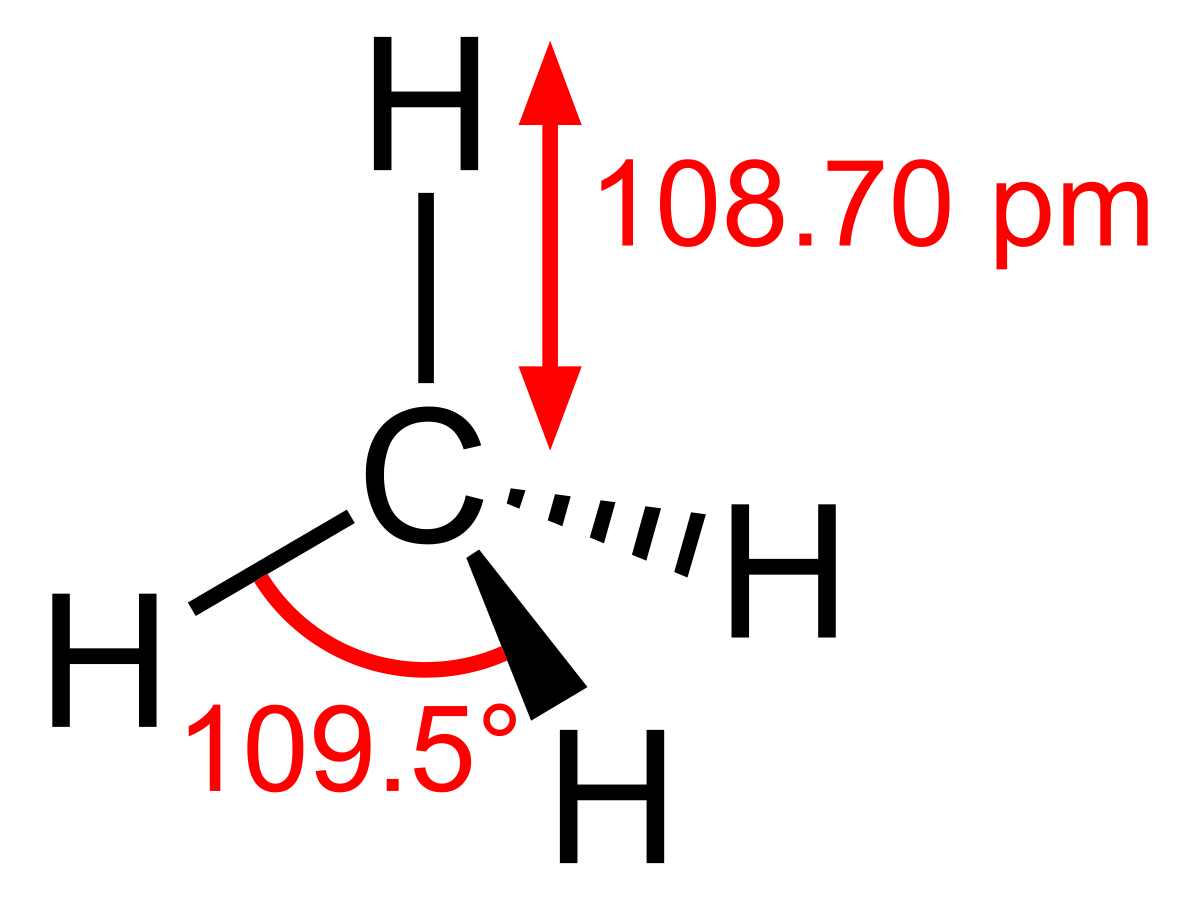
\includegraphics[width=8.75cm]{gambar/metana.png}
		\captionof{figure}{\textit{Senyawa Metana} \cite{Ben2016}}
	\end{center}

	Senyawa organik memiliki pola ikatan tunggal dan rangkap (rangkap dua dan tiga) karena karbon memiliki 4 elektron valensi yang menyebabkan karbon dapat berikatan dengan 4 buah unsur yang berbeda \cite{Clayden2012}. Kimia organik sangatlah berguna untuk produk komersial dan juga produk sains. Seperti contohnya untuk kosmetik, pelumas, bahan petrokimia dan lainnya. Salah satu senyawa kimia organik yang saat ini sedang diteliti yaitu senyawa Graphene.
	
	\section{Graphene}
	Graphene merupakan senyawa dengan ketebalan seperti ketebalan satu buah atom (\textit{one-atom-thick}) dan berstruktur 2 dimensi yang terdiri dari miliaran atom karbon (C) yang terbentuk seperti kisi heksagonal (atau sering disebut dengan sarang lebah) dan merupakan struktur fundamental untuk setiap bentuk karbon saat ini \cite{Clemons2010}\cite{Sahu2017}. Senyawa graphene memiliki karakteristik tebal yang sangat tipis, fleksibel, kuat dan transparan \cite{Ni2015}. Graphene lebih keras daripada intan, namun lebih elastis daripada karet, lebih kuat daripada baja dan lebih ringan daripada aluminium \cite{Berger2019}. Graphene merupakan turunan dari karbon yang dijadikan lembaran dan berasal dari graphite.
	
	\begin{center}
		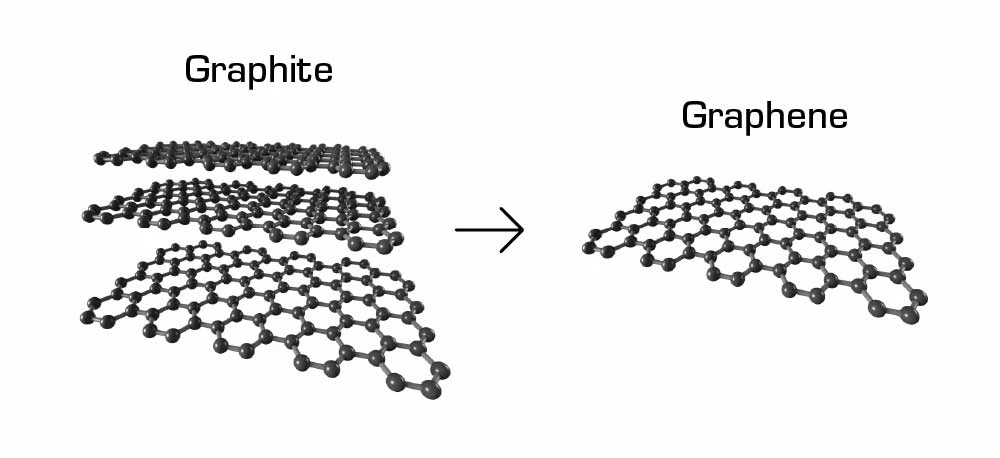
\includegraphics[width=8.75cm]{gambar/grafit.png}
		\captionof{figure}{\textit{Struktur Graphene dan Graphite} \cite{Verjari}}
	\end{center}
	
	Graphene hanya terdiri dari atom C yang jarak antar atom C sebesar ± 0.142 nm \cite{Zhen2017} dan jarak interplanar nya 0.335 nm. Setiap atom karbon (atom C) memiliki radius $\pm$ 170 pm atau 0.17 nm (\textit{Van der Walls radius}) \cite{10.1088/2053-2563/ab35d1ch1}. Graphene memiliki mobilitas elektron lebih dari 15000 $ cm^2 V^{-1} s^{-1} $. Dari sini bisa disimpulkan bahwa Graphene memiliki sifat kimia dan fisiknya yang sangat baik. Lalu karena Graphene adalah dasar dari alotrop grafit, lalu dapat dibentuk menjadi fullerene 0D, digulung menjadi tabung nano (nanotube) 1D, dan ditumpuk menjadi grafit 3D, inilah sebabnya Graphene disebut sebagai induk dari grafit \cite{Chakraborty2018}.
		
	\begin{center}
	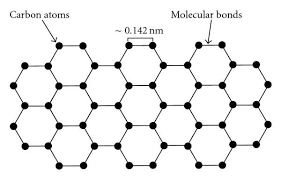
\includegraphics[width=8cm]{gambar/grafen.png}
	\captionof{figure}{\textit{Struktur Senyawa Graphene} \cite{Clemons2010}}
	\end{center}
	
	Aplikasi dari Graphene bisa digunakan menjadi resonator, saklar, katup, konduktor dan beberapa aplikasi lainnya \cite{Clemons2010}.
	
	\begin{center}
		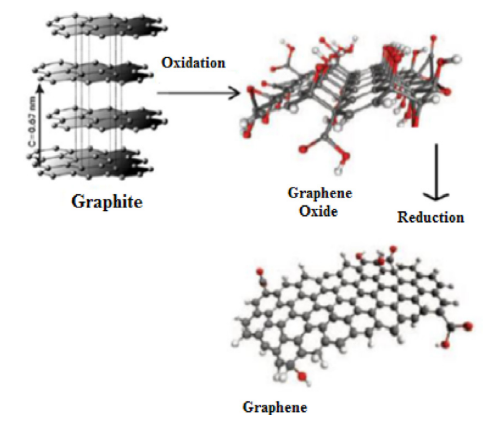
\includegraphics[width=8cm]{gambar/oksgraf.png}
		\captionof{figure}{\textit{Pembuatan Graphene dari Graphite} \cite{Korkmaz2020}}
	\end{center}
	
	Karakteristik dari Graphene bisa kita lihat, salah satunya mengenai energi yang dimiliki oleh orbital molekul Graphene. Untuk melihat energinya, kita dapat menggunakan suatu teori yang dikemukakan oleh Enrich Hückel yang bernama Teori Hückel. 
	
	\section{Teori Hückel}
	Teori Hückel sangat erat kaitannya dengan teori orbital molekul. Orbital molekul merupakan suatu penggambaran daerah yang dapat ditempati oleh suatu elektron dalam suatu molekul. Orbital molekul menggunakan pendekatan Schrödinger untuk elektron dalam medan listrik di inti atom suatu molekul. Dengan menggunakan orbital molekul kita bisa melihat konfigurasi elektron molekul. Karena orbital molekul merupakan fermion, maka ia akan memenuhi prinsip Pauli \cite{Coton1990}. Orbital dari suatu molekul memiliki level energinya masing-masing. Ikatan antar unsur dalam suatu molekul disebut ikatan-{$\sigma$}. Misalkan, senyawa {$C_2H_4$} (etilen), memiliki ikatan C=C dengan ikatan ganda, dan C-H dengan ikatan tunggal. Ikatan C=C dan C-H disebut ikatan-{$\sigma$}, dan karena hibridisasi dari etana memiliki elektron di {$2p_x$} dan {$2p_y$}, maka orbital di {$2p_z$} akan membentuk ikatan-{$\pi$}. Karena jarak antara ikatan-{$\pi$} dan ikatan-{$\sigma$} cukup jauh, menyebabkan interaksi antar ikatan {$\pi$} lebih besar daripada besar interaksi ikatan {$\sigma$} dan {$\pi$}. Maka kita bisa mengabaikan interaksi antara ikatan {$\sigma$} dan {$\pi$} \cite{Siregar2014}\\.
	\begin{center}
		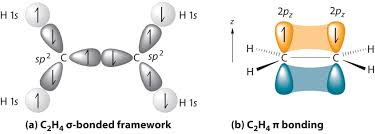
\includegraphics[width=11cm]{gambar/etilen.jpeg}
		\captionof{figure}{\textit{Orbital Molekul Etilen ({$C_2H_4$})} \cite{Anil}}
	\end{center}
	
	Dari sini, Hückel mengembangkan suatu teori dimana orbital molekul yang digunakan dapat dihitung energinya menggunakan teori elektron-{$\pi$}. Maka lahirlah Teori Orbital Molekul Hückel (Teori OMH) atau sering disebut dengan Teori Hückel. Dengan menggunakan teori Hückel, kita bisa melihat energi yang dihasilkan dari ikatan-{$\pi$} suatu molekul. Ia mengungkapkan bahwa orbital molekul yang dilambangkan oleh
	{$\psi$} adalah kombinasi linier dari orbital-orbital {$2p_z$} dari semua atom karbon dalam suatu molekul \cite{Rustaman2008}. Kombinasi linier orbital molekul sering disebut sebagai LCAO (\textit{Linear Combination of Atomic Orbital}) \cite{Maczynski1991}. LCAO {$2p_z$} ini dapat ditulis secara matematis dengan:
	\begin{equation}
	\label{lcao}
	{\psi} = \sum\limits_{i} c_i{\phi}_i
	\end{equation}
	dengan {$\phi_i$} adalah orbital {$2p_z$} dalam atom karbon ke-i. Jika $\hat{H}$ dianggap sebagai Hamiltonian efektif elektron-tunggal dalam molekul, maka berlaku:
	\begin{equation}
	\label{schrodinger}
	\hat{H}\psi = \epsilon\psi
	\end{equation}
	Persamaan \eqref{schrodinger} memenuhi persamaan sekuler:
	\begin{equation}
	\sum\limits_{j} {H_{ij}}-{\epsilon}{S_{ij}}c_j=0
	\end{equation}
	dengan
	\begin{equation}
	\label{hij}
	H_{ij} = \int {\phi_i}{\hat{H}}{\phi_j} \,dv
	\end{equation}
	\begin{equation}
	S_{ij} = \int {\phi_i}{\phi_j} \,dv
	\end{equation}
	Integral yang ada di persamaan \eqref{hij} bisa didefinisikan sebagai data empiris. Contohnya adalah {$H_{ii}$} adalah potensial ionisasi elektron-{$\pi$} di karbon ke-i dan {$H_{i,i{\pm}1}$} dalah energi yang dibutuhkan untuk elektron-{$\pi$} melompat ke atom terdekatnya. Karena {$S_{ii}=1$} dan {$S_{ij}$} jauh lebih kecil daripada 1 maka dapat diabaikan. Maka,
	\begin{equation}
	\label{alphabeta}
	\begin{cases}
	\alpha ; \  i = j
	\\
	H_{ij} = \beta ; \ j = i{\pm}1
	\\
	0 ; \ lainnya
	\end{cases}
	\end{equation}
	Singkatnya, persamaan \eqref{alphabeta} dapat menjadi sebuah persamaan matriks yang ditulis dengan,
	\begin{equation}
	\begin{bmatrix}
	{H_{11}-ES_{11}} & {H_{12}-ES_{12}} & ... &{H_{1j}-ES_{1j}}\\
	{H_{21}-ES_{21}} & {H_{22}-ES_{22}} & ... &{H_{2j}-ES_{2j}}\\
	... & ... & ... & ... \\
	{H_{i1}-ES_{i1}} & {H_{i2}-ES_{i2}} & ... &{H_{ij}-ES_{ij}}
	\end{bmatrix}
	\begin{bmatrix}c_1 \\ c_2 \\ ... \\ c_j \end{bmatrix} = 0
	\end{equation}
	Karena {$H_{ii} = \alpha$}, {$H_{ij} = \beta$}, dan {$S_{ij} = \delta_{ij} = 1$} jika {$i=j$} dan akan bernilai 0 jika {$i!=j$}. Maka matriks Hamiltoniannya menjadi,
	\begin{equation}
	\begin{bmatrix}
	\label{hamiltonian}
	\alpha - E & \beta & 0 &\beta \\
	\beta & \alpha - E & \beta & 0\\
	... & ... & ... & ... \\
	\beta & 0 & \beta & \alpha - E
	\end{bmatrix}
	\begin{bmatrix}c_1 \\ c_2 \\ ... \\ c_j \end{bmatrix} = 0
	\end{equation}
	Misalkan pada \textit{Ethylene} memiliki 2 atom C yang menyebabkan matriks Hamiltoniannya menjadi ukuran berukuran 2x2.
	\begin{equation}
	\begin{bmatrix}
	\alpha - E & \beta \\
	\beta & \alpha - E
	\end{bmatrix}
	\begin{bmatrix}c_1 \\ c_2 \end{bmatrix} = 0
	\end{equation}
	Energi orbital molekul dalam teori OMH didefinisikan dalam dua bentuk, yaitu energi dari sebuah elektron dalam orbital 2p (energi ionisasi) yang disebut dengan {$\alpha$} dan energi interaksi antara dua orbital 2p (energi resonansi) yang disebut dengan {$\beta$} \cite{Anil}\cite{Rustaman2008}.
	
	Dalam kasus ini, {$\hat{H}$} merupakan suatu matriks Hamiltonian yang menggambarkan keadaan orbital dari suatu molekul. Banyaknya atom karbon akan mempengaruhi besar matriks Hamiltonian yang didapat. Seperti misalkan benzene ({$C_6H_6$}) yang memiliki 6 atom karbon, maka matriks yang dihasilkannya berukuran 6x6.
	Jika dikaitkan dengan graphene yang memiliki jumlah atom C yang sangat banyak, maka matriks Hamiltonian yang dihasilkannya pun ukurannya akan sangat besar. Operasi yang akan digunakan yaitu operasi eigen. Hasil dari metode ini adalah energi orbital dari molekul uji yang digunakan. Aplikasi dari metode Hückel ini yaitu bisa menghitung celah pita \cite{Imamura2018}, rapat elektron dan konduktivitas bahan \cite{Siregar2014}. Dari literatur, dikatakan bahwa pada Graphene besar $\alpha$ = -10.7 eV dan $\beta$ = -1.58 eV \cite{Ni2015}.
	
	Sesuai persamaan Schrödinger tak bergantung waktu pada Persamaan \eqref{schrodinger}, maka kita bisa memperlakukan persamaan tersebut sebagai persamaan eigen. $\hat{H}$ sebagai operator, $\ket{\psi}$ sebagai fungsi gelombang, dan $\epsilon$ sebagai nilai eigen (\textit{eigen energy}). Tiap tingkatan eigen energy nya akan merepresentasikan keadaan energi dalam tiap orbital yang dimiliki oleh material tertentu. Sebelum menentukan lebar celah dari tingkat energi nya, perlu untuk memahami tentang teori pita terlebih dahulu.
	
	\section{Teori Pita}
	
	Dalam teori fisika zat padat, saat sebuah atom digabungkan dengan atom lainnya akan terjadi tumpang tindih fungsi gelombang elektron. Misalkan terdapat atom A dan B yang digabungkan. Jika tidak ada interaksi \textit{bonding} dan \textit{anti-bonding} nya, maka orbital yang dihasilkan adalah non ikatan, dimana elektron yang menempati orbital molekul terisi dan berenergi tinggi disebut \textit{Highest Occupied Molecular Orbital} (HOMO), dan orbital molekul tidak terisi dan berenergi paling rendah disebut \textit{Lowest Unoccupied Molecular Orbital} (LUMO) \cite{Risdiana2014}.
	\begin{center}
		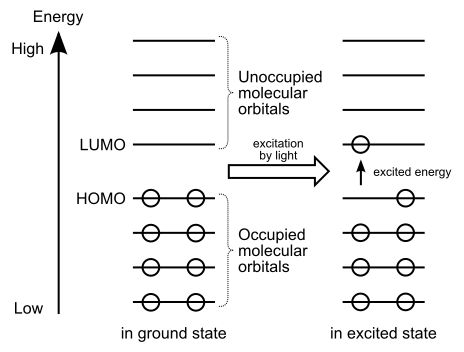
\includegraphics[width=9.1cm]{gambar/homolumo.png}
		\captionof{figure}{\textit{Diagram HOMO dan LUMO pada suatu molekul \label{homolumo}} \cite{Tomgelly2010}}
	\end{center}
	
	Teori pita adalah suatu model yang menjelaskan keadaan sebuah elektron yang hanya memiliki sebuah keadaan energi spesifik tertentu \cite{Anil}. Dalam sebuah senyawa, elektron akan menempati suatu tempat sesuai energi spesifik yang dimilikinya. Tempat inilah yang akan disebut sebagai pita energi. Sesuai dengan larangan Pauli (\textit{Pauli Exclusion}) dimana tidak ada dua elektron yang memiliki bilangan kuantum yang sama. Jika terdapat elektron lain, elektron tersebut akan membuat pita baru dan tidak akan menempati keadaan pita yang lainnya \cite{Faizi2021}.
	
	\section{Spektrum Absorbansi}
	
	Pada Gambar \ref{homolumo}, saat terdapat cahaya berenergi tertentu ditembakkan, maka orbital yang berada di daerah HOMO akan memiliki energi berlebih. Akibatnya, orbital tersebut akan tereksitasi ke keadaan dengan energi yang lebih tinggi. Karena orbital tersebut tidak stabil saat berada di keadaan energi yang bukan keadaan asalnya, orbital tersebut akan de-eksitasi kembali ke keadaan awalnya dengan meng-emisikan energi berlebih yang ia serap menjadi suatu gelombang emisi \cite{Bird2002}. Dari fenomena tersebut, kita bisa mengetahui celah pita yang dimiliki oleh senyawa tertentu dan bisa melihat energi yang di serap di tiap celah energinya dengan menggambarkan spektrum absorbansinya. Spektrum Absorbansi mengacu pada pengukuran penyerapan radiasi (melalui spektroskopi) sebagai fungsi energi atau panjang gelombang pada sebuah sampel. Untuk mencari absorbansi terhadap perubahan energi eksitasinya dapat menggunakan persamaan,
	
	\begin{equation}
	\label{absorbansi}
	\tilde{G}(E) = \frac{1}{N} \sum\limits_{i}^N |\tilde{G}^{(j)}|^{2}\delta_{E,E_{j}}
	\end{equation}
	dengan
	\begin{equation}
		\tilde{G}^{(j)} = g\sum\limits_{i}^N \bra{\upvarphi_0}\hat{\sigma}_{eg}^{(i)}+\hat{\sigma}_{ge}^{(i)}\ket{\upvarphi_j}
	\end{equation}
	$\delta_{E,E_{j}}$ adalah delta \textit{kronecker} dan $E_{j}$ adalah \textit{eigen energy} pada keadaan kolektif \cite{Abdussalam2017}. 
	
	Permasalahan yang dihadapi adalah ukuran matriks Hamiltonian yang sangat besar dan ini berefek pada laju komputasi yang akan kita lakukan. Hal tersebut bisa membuat laju komputasi menurun drastis karena proses komputasi yang sangat banyak dan tidak bisa dilakukan secara paralel. Untuk menjawab permasalahan tersebut, maka kita akan menggunakan operasi Block Matrix sebagai paralelisasi operasi matriks agar dapat dikerjakan dengan worker yang berbeda dan membantu dalam komputasi.
	
	\section{\textit{Block Matrix}}

	\textit{Block Matrix} merupakan salah satu operasi yang paling penting untuk meningkatkan kinerja komputasi. Dengan menggunakan Block Matrix maka operasi dapat diparalelisasi \cite{Davis2004}. Block Matrix adalah operasi matriks dimana suatu matriks berdimensi besar akan dibagi menjadi beberapa sub matriks kecil \cite{Ford2003}.
	
	\begin{center}
		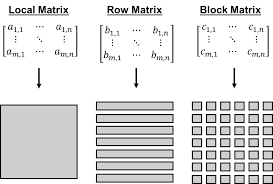
\includegraphics[width=9.1cm]{gambar/blockmat.png}
		\captionof{figure}{\textit{Perbandingan Local Matrix, Row Matrix dan Block Matrix} \cite{Pisciuneri2016}}
		\label{blockmatrix}
	\end{center}
	
	Terlihat dari Gambar \ref{blockmatrix} bahwa Block Matrix akan membagi matriks yang awalnya berukuran sangat besar (yaitu Local Matrix), menjadi beberapa sub matriks kecil. Misalkan kita memiliki matriks A dengan ukuran 4x4,
	\begin{equation}
	A = 
	\begin{bmatrix}
	\label{submat}
	a_{11} & a_{12} & a_{13} & a_{14} \\
	a_{21} & a_{22} & a_{23} & a_{24} \\
	a_{31} & a_{32} & a_{33} & a_{34} \\
	a_{41} & a_{42} & a_{43} & a_{44}
	\end{bmatrix}
	\end{equation}
	dengan menggunakan Block Matrix, maka matriks A dapat kita bagi menjadi 4 sub matriks yaitu {$A_{11}, A_{12}, A_{21}, A_{22}$}.
	\begin{equation}
	A = 
	\begin{bmatrix}
	A_{11} & A_{12} \\
	A_{21} & A_{22}
	\end{bmatrix}
	\end{equation}
	jika ditulis per submatriksnya menjadi,
	\begin{equation}
	A_{11} = 
	\begin{bmatrix}
	a_{11} & a_{12} \\
	a_{21} & a_{22}
	\end{bmatrix}
	A_{12} = 
	\begin{bmatrix}
	a_{13} & a_{14} \\
	a_{23} & a_{24}
	\end{bmatrix}
	A_{21} = 
	\begin{bmatrix}
	a_{31} & a_{32} \\
	a_{41} & a_{42}
	\end{bmatrix}
	A_{22} = 
	\begin{bmatrix}
	a_{33} & a_{34} \\
	a_{43} & a_{44}
	\end{bmatrix}
	\end{equation}
	Salah satu metode Block Matrix adalah dengan menggunakan \textit{Schur Decomposition}. Dekomposisi Schur akan membagi sebuah matriks menjadi 4 buah sub matriks dan menghitung determinan tiap sub matriksnya \cite{Gallier2010}. Jika menggunakan persamaan \eqref{submat}, maka dekomposisi Schur nya menjadi
	\begin{equation}
	\label{schur}
	det\begin{bmatrix}
	A_{11} & A_{12} \\
	A_{21} & A_{22}
	\end{bmatrix} = 
	det(A_{11}) * det(A_{22}-A_{21}A_{11}^{-1}A_{12})
	\end{equation}
	
	Karena elemen matriks yang didapatkan dari Graphene sangat banyak, dan diperlukan adanya sistem komputasi yang bisa memproses banyak data dengan kecepatan yang sangat tinggi. Maka kita akan menggunakan suatu metode menggunakan Big Data.
	
	\section{\textit{Big Data}}
	
	\begin{center}
		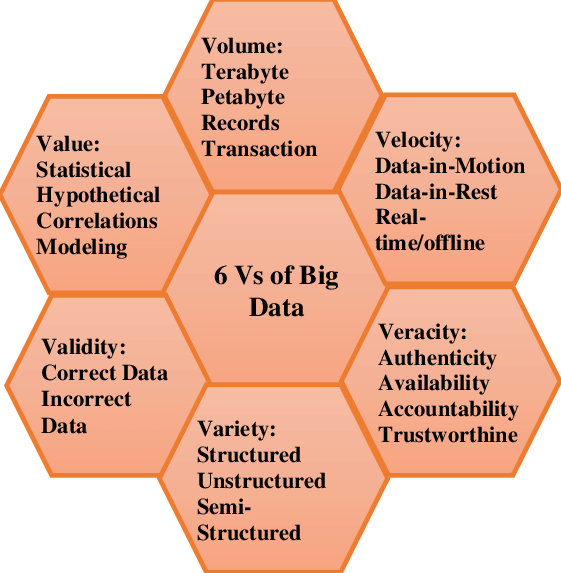
\includegraphics[width=7cm]{gambar/bigdat.png}
		\captionof{figure}{\textit{Big Data dan Karakteristiknya} \cite{Saqlain2017}}
	\end{center}

	\textit{Big Data} adalah salah satu metode cara memproses berbagai jenis data atau dalam literatur lain dikatakan bahwa \textit{Big Data} adalah data yang berisi lebih banyak variasi yang datang dalam volume yang terus meningkat dan dengan kecepatan meningkat juga \cite{Oracle2020}. Data dibagi menjadi dua tipe, yaitu Data Terstruktur (data numerik), dan Data Tidak Terstruktur (teks, suara, gambar, dll) \cite{Shakhovska2019}. Secara makna, Big Data merupakan suatu data yang ukurannya sangat besar, bentuk yang tidak teratur, dengan komunikasi data kecepatan tinggi. Big Data memiliki 6 karakteristik yang disebut sebagai “\textit{6V’s of Big Data}” yang tertera pada Tabel 2.1.
	
	\begin{table}[h]
		\centering
		\caption{Karakteristik Big Data \cite{Moura2015}\cite{Schaafsma2020}}
		\label{tab:my_label}
		\begin{tabular}{|p{0.2\linewidth} | p{0.7\linewidth}|} 
			\hline
			Volume\centering & Volume adalah salah satu hal yang menjadi feature dari Big Data. Berkaitan dengan hubungan antara ukuran dan kapasitas pemrosesan. \\ \hline
			Velocity\centering & Kecepatan pemrosesan Big Data sangatlah cepat, ini dikarenakan dari data yang dimilikinya sangat besar dan akan semakin membesar seiring banyaknya data yang masuk. Kecepatan yang dimiliki sangat cepat karena memanfaatkan data geolokasi, tren dan informasi input data. \\ \hline
			Value\centering & Value menjelaskan bahwa nilai yang akan diperoleh dari suatu data dan lebih bernilai dari stored data \\ \hline
			Variability\centering & Variability mengungkap tentang variable-variabel yang mempengaruhi proses komunikasi data dan pemrosesannya beserta kemungkinan terbaiknya. \\ \hline
			Veracity\centering & Veracity menunjukkan kualitas dan asal data, dan sebagai penyeleksian kebenaran dan keaslian data. \\ \hline
			Variety\centering & Variety menggambarkan bahwa didalam Big Data terdapat banyak variasi atau macam data yang akan diproses dan dianalisis. Bise berupa data numerik, audio video, bahkan teks. \\ \hline
		\end{tabular}
	\end{table}

	Big Data biasa disebut sebagai Not-Only Structured Query Language (NoSQL), hal ini berbeda dengan Relational Database Management System (RDBMS) atau basis data tradisional mulai dari variasi data untuk NoSQL bisa mencakup data semi terstruktur dan data tidak terstruktur, kecepatan baca-tulis (Read-Write) data dari Big Data yang sangat cepat (bergantung pada jumlah node) dan scalable \cite{Fadillah2020}.
	\begin{center}
	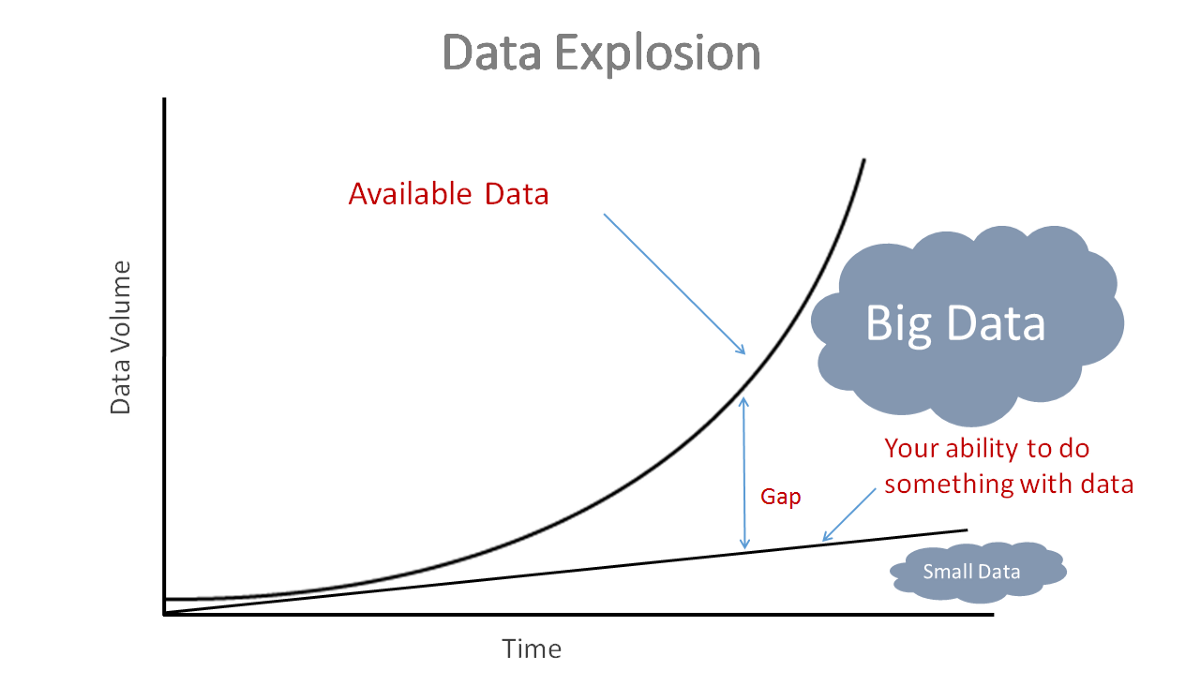
\includegraphics[width=9cm]{gambar/perform.png}
	\captionof{figure}{\textit{Grafik Ledakan Data terhadap Waktu Komputasi} \cite{Stewart2019}}
	\end{center}
	Beberapa kelebihan dan kekurangan jika menggunakan Big Data terdapat pada Tabel 2.2.
	
	\begin{table}[htb]
		\centering
		\caption{Kelebihan dan Kekurangan Big Data \cite{Harvey2018}}
		\begin{tabular}{|P{0.5\linewidth} | P{0.5\linewidth}|}
			\hline
			\textbf{Kelebihan} & \textbf{Kekurangan} \\ \hline
			Pengambilan keputusan yang lebih baik & Kebutuhan akan \textit{talent} yang profesional di bidangnya \\ \hline
			Peningkatan produktivitas & Kualitas data \\ \hline
			Mengurangi biaya & Perlunya perubahan budaya untuk menggunakan Big Data \\ \hline
			Peningkatan layanan pelanggan & Peraturan yang mengatur tentang privasi data \\ \hline
			Deteksi penipuan & Resiko keamanan \\ \hline
			Peningkatan pendapatan & Perubahan yang cepat \\ \hline
			Peningkatan agility & Kebutuhan perangkat keras pendukung \\ \hline
			Inovasi yang lebih besar & Kecepatan lebih cepat dalam pemrosesannya  \\ \hline
			Kecepatan lebih cepat dalam pemrosesannya & Biaya\\ \hline
		\end{tabular}
	\end{table}

	Terdapat beberapa \textit{platform} yang sering digunakan dalam pengolahan Big Data, dan beberapa dan yang akan digunakannya adalah Apache Spark.
	
	\subsection{\textit{Apache Spark}}
	\begin{center}
		
\includegraphics[width=7.5cm]{gambar/spark.png}
		\captionof{figure}{\textit{Apache Spark} \cite{Apache2018}}
	\end{center}
	
	Apache Spark merupakan sebuah aplikasi mesin analitik yang terpadu untuk pemrosesan data berskala besar \cite{Apache2018}. Apache Spark banyak digunakan di berbagai industri, seperti Netflix, Yahoo, dan eBay. Bahasa yang dapat digunakan dalam Apache Spark adalah \textit{Scala}, \textit{SQL} dan \textit{Python}. Arsitektur data dari Spark berupa RDD (\textit{Resilient Distributed Dataset}). \textit{Resilient} berarti toleran terhadap kesalahan dan dapat membuat data baru dari kesalahan tersebut, \textit{Distributed} berarti data didistribusikan di antara beberapa node dalam sebuah cluster, dan \textit{Dataset} berarti Kumpulan data yang berisi suatu nilai \cite{Chand2020}.
	\begin{center}
		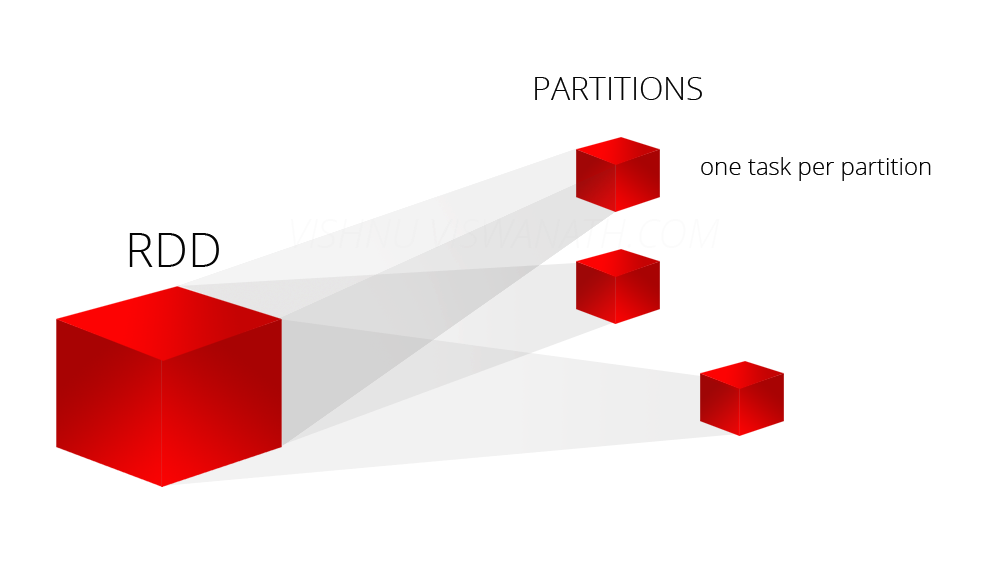
\includegraphics[width=7.5cm]{gambar/rdd.png}
		\captionof{figure}{\textit{Contoh Kasus RDD pada Spark} \cite{Kumar2018}}
		\label{rdd}
	\end{center}
	Dengan menggunakan RDD, kita bisa melakukan beberapa hal seperti:
	\begin{enumerate}
		\item \textit{Transformations} = Operasi ini dapat digunakan untuk membuat RDD baru
		\item \textit{Actions} = Operasi ini diaplikasikan pada RDD untuk menginstruksikan Apache Spark untuk menerapkan komputasi dan meneruskan hasilnya kembali ke driver
	\end{enumerate}
	Kelebihan dari Spark adalah:
	\begin{enumerate}
		\item Kecepatan\\
		Spark memiliki kecepatan 100x lebih cepat daripada Hadoop. Ini karena Spark menggunakan komputasi dan beberapa pengoptimalan lainnya. 
		\item Kemudahan dalam penggunaan\\
		Spark memiliki antarmuka yang mudah digunakan untuk memproses Big Data.
		\item Aplikasi terpadu\\
		Spark memiliki dukungan dan library yang sangat banyak, termasuk SQL, streaming data, machine learning, dan pemrosesan grafik. Salah satunya, spark dapat dioperasikan menggunakan library dari python yang disebut sebagai PySpark \cite{Databricks}.
	\end{enumerate}
	
	Apache Spark sangatlah cepat dalam pemrosesan data dikarenakan dalam kerjanya menggunakan \textit{In-Memory Processing} yang berarti semua pekerjaan atau pemrosesan data yang dilakukan oleh Apache Spark akan di proses di dalam \textit{memory}\cite{Bekker2017}. Untuk menggunakan fungsionalitas dari Spark, diperlukan \textit{SparkContext} sebagai titik masuk aplikasinya. Untuk skema alur data nya dapat dilihat di Gambar \ref{rdd} \cite{Tutorialspoint}.
	\begin{center}
		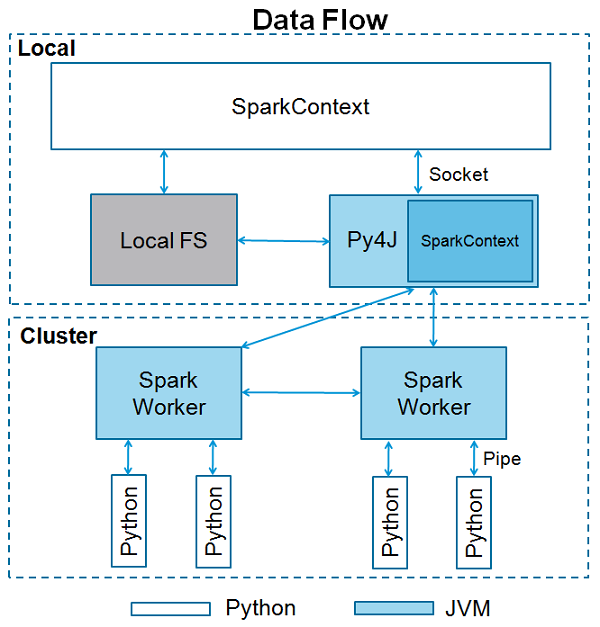
\includegraphics[width=6cm]{gambar/sparkcontext.png}
		\captionof{figure}{\textit{Alur Kerja Data pada Apache Spark} \cite{Tutorialspoint}}
	\end{center}

	Kegunaan Apache Spark atau lebih tepatnya PySpark pada penelitian ini adalah untuk memproses komputasi energi orbital dari Teori Hückel. Basis bahasa dari PySpark adalah Python, namun karena karakteristik yang dimiliki PySpark yang akan membuat komputasi nya akan semakin cepat dan dibandingkan dengan laju komputasi menggunakan Python biasa.
	
\chapter*{BAB III \\ METODE PENELITIAN}
\addcontentsline{toc}{chapter}{BAB III METODE PENELITIAN}
\setcounter{chapter}{3}
\setcounter{section}{0}
\setcounter{figure}{0}
\setcounter{equation}{0}
\thispagestyle{myplain}

Penelitian Kalkulasi Nilai Eigen berbasis Matriks Hamiltonian menggunakan Teknik \textit{Block Matrix} : Studi Kasus Pada \textit{Graphene} dilakukan dengan 3 tahapan, yaitu perancangan algoritma penelitian, perancangan kode komputasi dan simulasi data. Perancangan algoritma penelitian akan membuat cara kerja aplikasi yang akan dibuat dimulai dari \textit{Start} hingga komputasi berakhir. Dalam perancangan kode komputasi akan dibuat kode berbahasa \textit{Python} yang akan dieksekusi oleh \textit{Python Compiler} dan PySpark. Tahap terakhir adalah kalkulasi data data. Simulasi data akan mensimulasikan kode yang sudah dibuat menggnakan perangkat komputer dengan spesifikasi yang ditentukan. Dari hasil kalkulasi data ini akan dilihat hasil grafik celah energi dan spektrum absorbansi lalu performa komputasi yang dijelaskan dengan kecepatan komputasi yang dihasilkan dari variasi yang diterapkan.

	\section{Perancangan Algoritma Penelitian}
	
	Langkah-langkah penelitian dapat dilihat pada diagram alir penelitian pada Gambar \ref{diagram-alir} 
	\begin{center}
		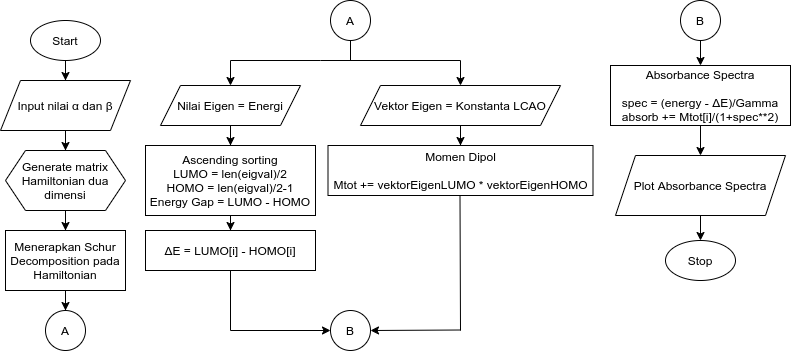
\includegraphics[width=13cm]{gambar/diagram.png}
		\captionof{figure}{Diagram Alir Penelitian}
		\label{diagram-alir}
	\end{center}
	 
	 Dalam penelitian ini, akan dilakukan dengan beberapa tahap, yaitu pendefinisian, pemecahan matriks utama menjadi sub matriks kecil, diagonalisasi matriks, dan subtitusi untuk dapat keluaran besar energi orbital molekul dari graphene dan laju konvergensi yang didapatkannya. Diawali dengan penginputan besar {$\alpha$} dan {$\beta$} dari Graphene lalu akan dibuat matriks Hamiltoniannya. Lalu, matriks Hamiltoniannya akan dioperasikan menggunakan dekomposisi Schur untuk dapat dikerjakan secara paralel. Keluaran nya berupa nilai eigen dan vektor eigen. Nilai eigen sebagai energi orbital, dan vektor eigen merupakan konstanta fungsi gelombangnya. Dari kedua keluaran ini, akan dicari besar absorpsi setiap perubahan energi eksitasinya lalu dibuatkan grafik.
	 
	\section{Alat yang Digunakan}
			\subsection{Perangkat Lunak}
			\begin{enumerate}
				\vspace{-0.2cm} \item \textit{Python} versi 3.8.5 
				\vspace{-0.8cm} \item \textit{Apache Spark} versi 3.0.1 dengan \textit{PySpark}
				\vspace{-0.8cm} \item \textit{Apache Hadoop} versi 3.14
				\vspace{-0.8cm} \item \textit{Visual Studio Code} versi 1.56.2
				\vspace{-0.8cm} \item \textit{Gnuplot} versi 5.4 \textit{patchlevel} 1
			\end{enumerate}
		
			\subsection{Perangkat Keras}
			\begin{enumerate}
				\vspace{-0.2cm} \item Server KST
				\begin{enumerate}
					\vspace{-0.8cm} \item Prosessor : Intel Xeon E3-1225; 4 Core @ 3.7 GHz
					\vspace{-0.8cm} \item RAM : 8 GB
					\vspace{-0.8cm} \item Sistem Operasi : Ubuntu 18.04 LTS
				\end{enumerate}
				\vspace{-0.8cm} \item Server Google Cloud Instance Iowa (US)
				\begin{enumerate}
					\vspace{-0.8cm} \item Prosessor : Intel Xeon Skylake; 4 vCore/vCPU @ 3.7GHz
					\vspace{-0.8cm} \item RAM : 16 GB
					\vspace{-0.8cm} \item Sistem Operasi : Ubuntu 20.04 LTS
				\end{enumerate}
			\end{enumerate}
	
	\section{Perancangan Kode Komputasi}
	\subsection{Perancangan Matriks Hamiltonian}
	
	Pada perancangan kode komputasi ini akan membuat kode dalam bahasa \textit{Python} yang akan dikonversi menjadi kode yang dapat dieksekusi di \textit{PySpark}. Matriks Hamiltonian yang dimiliki oleh Graphene bersifat matriks dua dimensi. Lalu dalam penentuan ikatan nya akan dilakukan menggunakan penentuan posisi atom acak dua dimensi. Penentuan posisi {$\vec{A}$} yaitu dengan
	\begin{equation}
	\vec{A} = A_x + A_y
	\end{equation}
	\begin{equation}
	A_x = rand * L_x
	A_y = rand * L_y
	\end{equation}
	dengan rand = angka acak, dan
	{$L_x$} = {$L_y$} = panjang horizontal dan vertikal.\\
	Untuk menentukan indeks cell dari matriks dapat menggunakan rumus:
	\begin{equation}
	index = A_y * L_x + A_x
	\end{equation}
	Maka, dari indeks yang dihasilkan akan menjadi matriks seperti berikut
	\begin{equation}
	\begin{bmatrix}
	index_{11} & index_{12} & index_{13} \\
	index_{21} & index_{22} & index_{23} \\
	index_{31} & index_{32} & index_{33}
	\end{bmatrix}
	\end{equation}
	atau jika dijadikan angka indeks,
	\begin{equation}
	\begin{bmatrix}
	9 & 8 & 7 \\
	6 & 5 & 4 \\
	3 & 2 & 1
	\end{bmatrix}
	\end{equation}
	angka indeks inilah yang akan digunakan dalam pembuatan fungsi matriks Hamiltonian.
	
	Kemudian karena kita akan mencari koordinat ({$index_x$}, {$index_y$}), maka kita harus mencari {$A_x$} dan {$A_y$} nya terlebih dahulu.
	\begin{equation}
	\begin{split}
	i_y = index_x / L_x \\
	i_x = index_x - i_y * L_x
	\end{split}
	\end{equation}
	Dari {$i_x$} dan {$i_y$} yang telah didapatkan, kemudian dicari {$index_j$} nya dengan rumus,
	\begin{equation}
	index_j = j_y * L_x + j_x
	\end{equation}
	dengan {$j_y = iy + dy$} dan {$j_x = ix + dx$}.
	
	Untuk menentukan atom mana saja yang terikat pada Graphene, kita bisa menurunkan dari ilustrasi pada Gambar \ref{struktur-graphene}.
	\begin{center}
		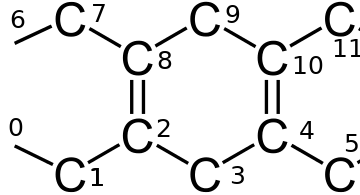
\includegraphics[width=7cm]{gambar/struk.png}
		\captionof{figure}{Indeks Struktur Empirik Graphene}
		\label{struktur-graphene}
	\end{center}
	Dari gambar terlihat bahwa tidak semua atom saling berikatan. Seperti contoh atom dengan indeks 1 tidak berikatan dengan atom indeks 7 dan hanya berikatan dengan atom indeks 0 dan 2. Lalu atom indeks 2 berikatan dengan indeks 1, 3 dan 8. Maka disini dilakukan pengondisian menggunakan vektor dengan rumus,
	\begin{equation}
	rad = \sqrt{dx^2 + dy^2}
	\end{equation}
	Hasil yang didapatkan digunakan untuk pengondisian dalam variabelisasi elemen $\alpha$ dan $\beta$ seperti pada persamaan \eqref{hamiltonian} dengan pengondisian sebagai berikut:
	
	\begin{equation}
	\begin{cases}
	rad = 0, \ H[i][j] = \alpha \\
	rad = 1, \ mod(L_x) = 0, \ abs(i-j) = L_x, \ dan mod(i) = 1, \ H[i][j] = 0 \\
	rad = 1, \ mod(L_x) = 1, \ mod(iy) = 0, \ abs(i-j) = L_x, \ dan mod(i) = 1, \ H[i][j] = 0 \\
	rad = 1, \ mod(L_x) = 1, \ mod(iy) = 1, \ abs(i-j) = L_x, \ dan mod(i) = 0, \ H[i][j] = 0 \\
	else, \ H[i][j] = \beta
	\end{cases}
	\end{equation}
	
	\subsection{Perancangan Kalkulasi Celah Energi}
	
	Matriks Hamiltonian yang didapat lalu diaplikasikan dengan teknik \textit{Block Matrix} dengan mnenggunakan dekomposisi Schur. Dengan mengaplikasikan persamaan \eqref{schur}, akan didapatkan dua buah output yaitu nilai eigen dan vektor eigen. Nilai eigen akan menjadi energi orbital, dan vektor eigen akan menjadi koefisien fungsi gelombangnya (yaitu c pada persamaan \eqref{lcao}).
	
	Energi orbital nya akan di urutkan secara \textit{ascending} untuk menempatkan energi sesuai konsep HOMO dan LUMO. Setengah atas adalah HOMO, dan setengah bawah adalah LUMO. Untuk mencari celah pita nya, dapat menghitung perbedaan energi HOMO dan LUMO terluarnya,
	\begin{equation}
	E_{gap} = E_{LUMO \ terluar} - E_{HOMO \ terluar} \ (eV)
	\end{equation}
	
	\subsection{Perancangan Kalkulasi Celah Energi dengan \textit{Python} dan \textit{PySpark}}
	
	Untuk mencari celah energi nya, akan dilakukan menggunakan 2 buah aplikasi yaitu \textit{Python} dan \textit{PySpark}. Untuk Python akan dilakukan dengan 3 variasi yaitu \textit{Serial Processing}, \textit{Multi Processing}, dan \textit{Threading}. Dari 4 buah variasi komputasi ini, akan dilihat performa komputasinya melalui jumlah waktu yang dibutuhkan untuk memproses matriks Hamiltonian. Khusus untuk PySpark, akan dijalankan menggunakan (\lstinline{spark-submit}) dengan 4 core di setiap workernya. Skema kerja dari PySpark adalah sebagai berikut:
	
	\begin{center}
		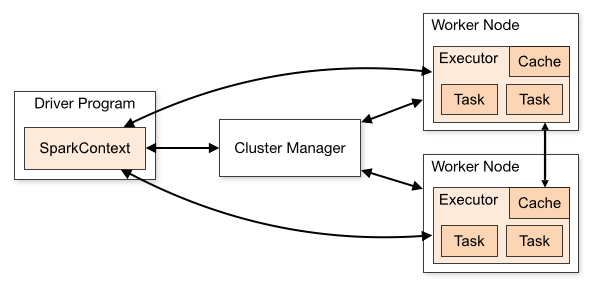
\includegraphics[width=10cm]{gambar/skem.png}
		\captionof{figure}{Skema Kerja PySpark}
		\label{sparkworker}
	\end{center}
	Dalam Gambar \ref{sparkworker} terlihat bahwa Spark menggunakan arsitektur master / slave. Spark memiliki satu koordinator pusat (\textit{driver}) yang berkomunikasi dengan banyak \textit{worker} (eksekutor) yang tersebar. \textit{Driver} dan setiap \textit{worker} menjalankan proses Python mereka masing-masing.
	
	\subsection{Perancangan Kalkulasi Absorbansi terhadap Perubahan Energi Eksitasi}
	
	Hasil dari kalkulasi energi eigen, lalu akan dihitung besar energi eksitasi dari HOMO ke LUMO dengan mengurangi tiap orbital LUMO dengan HOMO nya
	\begin{equation}
	\label{deltaE}
	\Delta E = E_{LUMO} - E_{HOMO} \ (eV)
	\end{equation}
	
	Untuk vektor eigen nya, dioperasikan untuk mencari momen dipol yang dimiliki oleh Graphene dengan mengalikan tiap kolom di daerah LUMO dengan tiap kolom di daerah HOMO. Secara matematisnya,
	\begin{equation}
	\label{dipol}
	M_{total} = \sum\limits_{i}^{N_{atoms}} {c_{[i,\ LUMO]}}*{c_{[i,\ HOMO]}}
	\end{equation}
	
	Dengan menggabungkan hasil dari $\Delta E$ pada persamaan \eqref{deltaE} dengan $M_{total}$ pada persamaan \eqref{dipol}, maka kita dapat mencari nilai absorbansinya dengan menggunakan persamaan \eqref{absorbansi}.
	
\chapter*{BAB IV \\ HASIL DAN PEMBAHASAN}
\addcontentsline{toc}{chapter}{BAB IV HASIL DAN PEMBAHASAN}
\setcounter{chapter}{4}
\setcounter{section}{0}
\setcounter{figure}{0}
\setcounter{equation}{0}
\thispagestyle{myplain}

\section{Hasil Kode Komputasi}

Pada bab ini, akan membahas mengenai hasil dari perancangan kode komputasi, seperti kalkulasi celah energi, kalkulasi celah energi dengan \textit{Python} dan \textit{PySpark} dan kalkulasi absorbansi terhadap perubahan energi eksitasi.

\subsection{Hasil Matriks Hamiltonian}

Dari perancangan matriks Hamiltonian, akan didapatkan sebuah matriks $m_{x}n$ 2 dimensi. Matriks ini akan menjelaskan keberadaan partikel dan ikatan yang dimiliki oleh partikel tersebut dengan tetangga terdekatnya. Karena hanya mengambil tetangga terdekatnya, maka jarak antar atomnya dapat dianggap satu ($r_{ij}=1$). Untuk membuat matriks Hamiltoniannya, maka harus terlebih dahulu menentukan panjang atom di sumbu x dan panjang atom di sumbu y. 
\begin{center}
	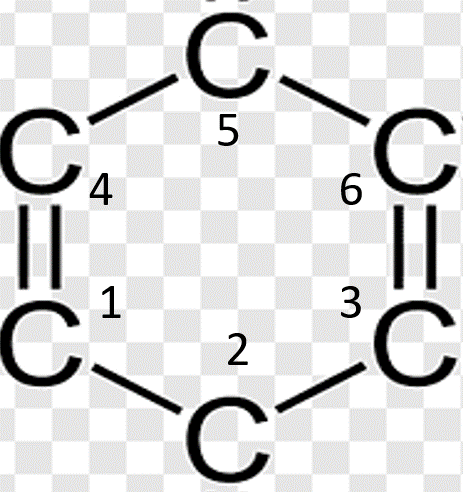
\includegraphics[width=5cm]{gambar/benzene.png}
	\captionof{figure}{Struktur Empirik Benzene untuk Hückel}
	\label{benzene_structure}
\end{center}
Untuk benzene, maka panjang atom x nya adalah 3, dan panjang atom y nya adalah 2. Matriks Hamiltonian yang didapatkan nya seperti berikut.
\begin{center}
	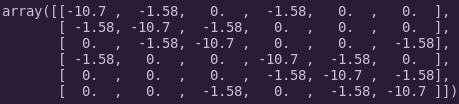
\includegraphics[width=10cm]{gambar/benzene-hamiltonian.png}
	\captionof{figure}{Matriks Hamiltonian Benzene}
	\label{benzene_hamilton}
\end{center}

Jika kita validasi Gambar \ref{benzene_hamilton} dengan ikatan benzene pada Gambar \ref{benzene_structure}, maka terlihat bahwa tidak semua atom akan berikatan satu sama lain. Jika mengambil contoh atom $C_1$, maka hanya akan berikatan dengan atom $C_4$ dan $C_2$. Maka atom $C_1$ akan bernilai $\alpha$ dan ikatan dengan atom $C_4$ dan $C_2$ bernilai $\beta$. Maka matriks dengan indeks $H_{11}$ bernilai $-10,7$ eV, lalu $H_{12}$ dan $H_{14}$ bernilai $-1,58$ eV, begitupun untuk indeks lainnya.

Untuk atom karbon, jika diperbanyak, maka indeks ikatannya pun akan berbeda. Misalkan untuk senyawa $C_{10}$, struktur yang dimilikinya akan seperti berikut,
\begin{center}
	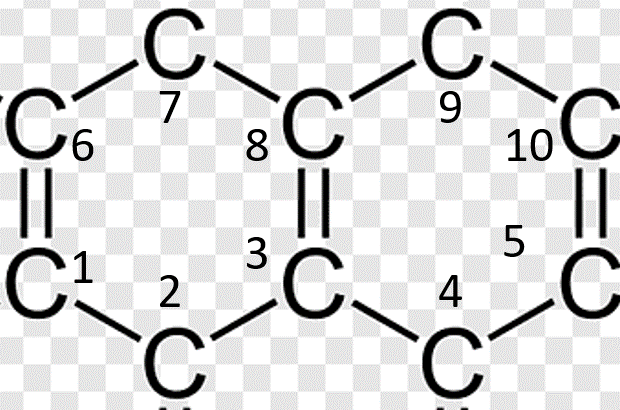
\includegraphics[width=6cm]{gambar/C10.png}
	\captionof{figure}{Struktur Empirik $C_{10}$ untuk Hückel}
	\label{c10_structure}
\end{center}
dan matriks hamiltonian yang didapatkannya adalah
\begin{center}
	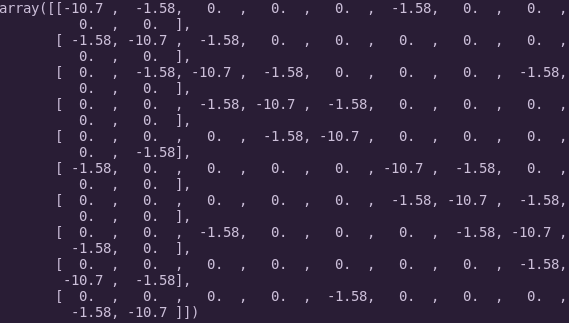
\includegraphics[width=10cm]{gambar/c10_hamiltonian.png}
	\captionof{figure}{Matriks Hamiltonian $C_{10}$}
	\label{c10_hamilton}
\end{center}
dan jika kita menggunakan Graphene dengan besar 3.5 nm atau setara 21 atom karbon, maka akan dihasilkan matriks hamiltonian,
\begin{center}
	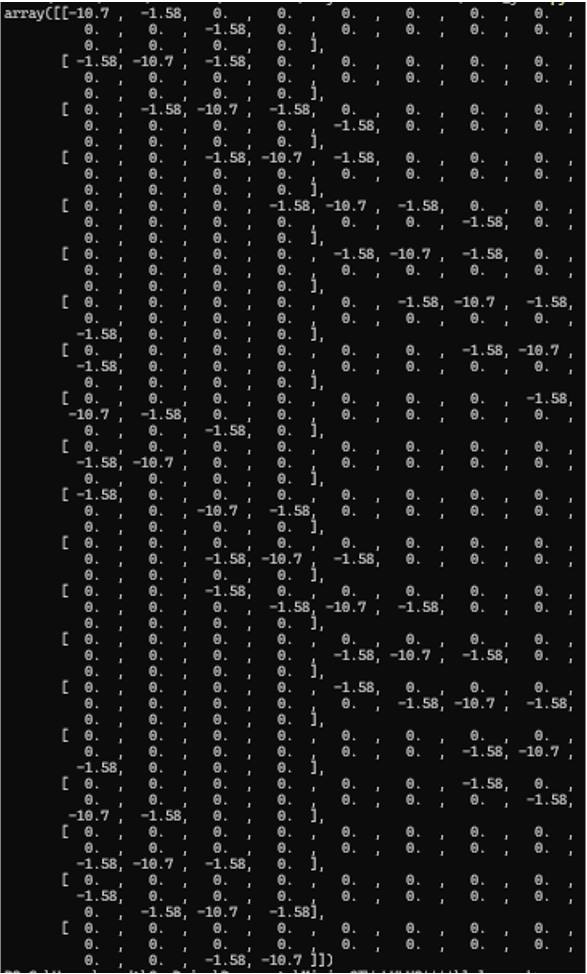
\includegraphics[width=7.5cm]{gambar/graphene21_hamiltonian.png}
	\captionof{figure}{Matriks Hamiltonian Graphene dengan 21 Atom}
	\label{graphene21_hamilton}
\end{center}
Terlihat antara struktur $C_{10}$ (Gambar \ref{c10_structure}) dengan matriks hamiltoniannya (Gambar \ref{c10_hamilton}) memiliki indeks yang sama. Sebagai contoh, untuk atom $C_{3}$ akan berikatan dengan atom $C_{8}$, $C_{2}$ dan $C_{4}$ yang menyebabkan terdapat nilai $\beta$ pada matriks $H_{38}$. $H_{34}$ dan $H_{32}$. Sedangkan untuk atom $C_{2}$ hanya berikatan dengan atom $C_{1}$ dan $C_{3}$ saja yang menyebabkan nilai $\beta$ hanya terdapat pada matriks $H_{21}$ dan $H_{23}$.

Karena hanya melibatkan ikatan dengan tetangga terdekat (\textit{First-Nearest Neighbor}) sesuai asumsi Hückel, maka nilai $\beta$ (sebesar $-1.58$ eV) hanya untuk ikatan terdekatnya, sedangkan interaksi dengan atom lainnya diabaikan.

\subsection{Hasil Kalkulasi Celah Energi}

Dari matriks Hamiltonian yang didapatkan, kemudian dihitung nilai eigen nya. Nilai eigen ini yang menjadi energi yang dimiliki tiap orbital molekul. Nilai energi orbital molekul dari benzene adalah,
\begin{center}
	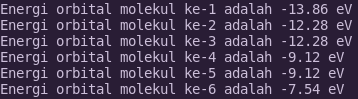
\includegraphics[width=8cm]{gambar/benzene-energy.png}
	\captionof{figure}{Energi Orbital Molekul Benzene}
	\label{benzene_energy}
\end{center}
dengan mengurangi energi HOMO terluar dengan LUMO terluar, maka didapatkan nilai celah energinya.
\begin{equation}
E_{gap} (benzene) = (-9,12 - (-12,28)) eV = 3,16 \ eV
\end{equation}
Jika dibandingkan dengan hasil literatur, yaitu sebesar $3.1$ eV \cite{Masiak2017}, maka terdapat kesalahan relatif sebesar 18,96\%.

Apabila jumlah atom karbon ditambah menjadi senyawa Graphene dengan 21 atom, maka energi orbital molekul nya menjadi 21 keadaan dengan energi tiap keadaannya sebesar,
\begin{center}
	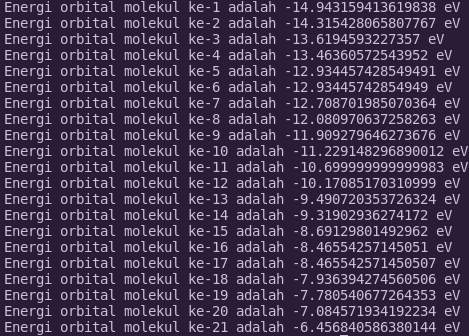
\includegraphics[width=8cm]{gambar/graphene21_energy.png}
	\captionof{figure}{Energi Orbital Molekul Graphene dengan 21 Atom}
	\label{graphene21_energy}
\end{center}
dengan celah energi nya sebesar 0.5291 eV. Dalam literatur, untuk Graphene berukuran 3.5 nm atau setara dengan 21 atom karbon memiliki celah energi 0,4 eV \cite{Jeon2013}. Kesalahan relatif yang didapatkan sebesar 32,28 \%. Kesalahan relatif ini terjadi karena Teori Hückel merupakan persamaan semi-empirik dengan pendekatan nilai $\alpha$ dan $\beta$. Maka akan terdapat perbedaan nilai dengan hasil dari karakterisasi bahan tersebut, dan juga karena Teori Hückel mengabaikan interaksi dengan atom-atom lainnya yang menyebabkan tidak semua atom akan saling berinteraksi pada teori ini.

Lalu, terlihat bahwa jika jumlah atom karbon diperbanyak, perbedaan energi tiap orbitalnya akan mengecil. Ini menyebabkan celah energinya pun akan semakin mengecil. Saat di plot kedalam grafik, maka akan terlihat jelas penurunan celah energinya seperti pada Gambar \ref{bandgap} dan pada Tabel \ref{gaptable}
\begin{table}[h]
	\centering
	\caption{Tabel Celah Energi terhadap Banyaknya Atom Karbon}
	\label{gaptable}
	\begin{tabular}{|c|c|} 
		\hline
		N (atom) & Celah Energi (eV)\\ \hline
		6 & 3,1599 \\ \hline
		21 & 0,5291 \\ \hline
		22 & 0,6942 \\ \hline
		36 & 0,3284 \\ \hline
		100 & 0,1306 \\ \hline
		196 & 0,0698 \\ \hline
		324 & 0,0434 \\ \hline
		484 & 0,0296 \\ \hline
		676 & 0,0214 \\ \hline
		900 & 0,0163 \\ \hline
		... & ... \\ \hline
		8100 & 0.0019 \\ \hline
		8836 & 0,0017 \\ \hline
		9604 & 0,0016 \\ \hline
	\end{tabular}
\end{table}
\begin{center}
	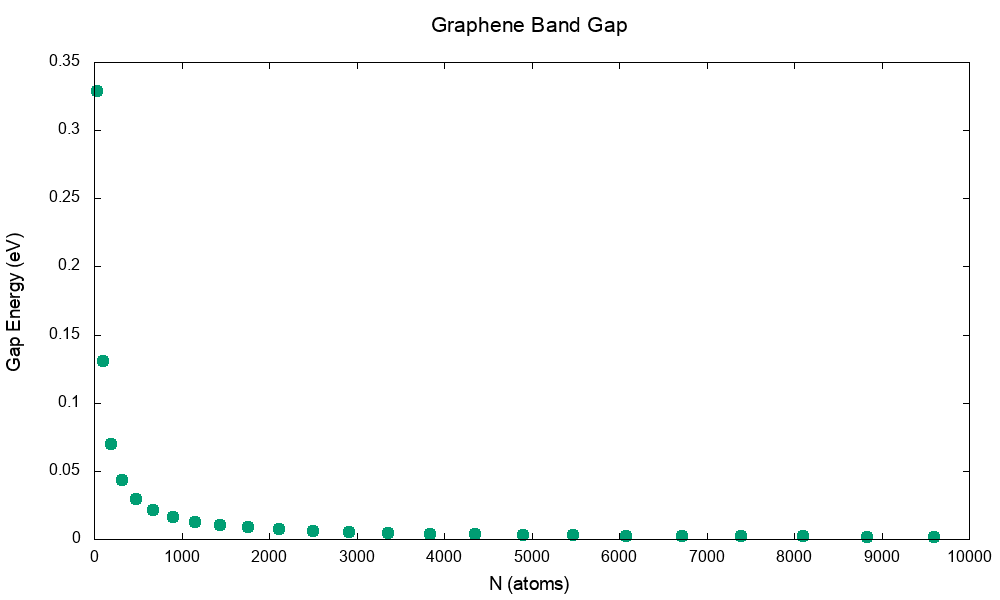
\includegraphics[width=12cm]{gambar/bandgap.png}
	\captionof{figure}{Grafik Celah Energi terhadap Banyaknya Atom}
	\label{bandgap}
\end{center}

\subsection{Hasil Kalkulasi Celah Energi dengan \textit{Python} dan \textit{PySpark}}

Karena ukuran matriks yang sangat besar, maka dilakukanlah beberapa teknik untuk mencari pemrosesan komputasi dengan waktu tercepat. Untuk itu, dilakukanlah komputasi dengan Python (menggunakan \textit{Serial Processing}, \textit{Multiprocessing}  dan \textit{Threading}) dan PySpark. Dengan menggunakan matriks berukuran $36 * 36$ hingga $4900 * 4900$, didapatkan data waktu pemrosesan untuk Server Google Cloud dan Server KST sebagai berikut,
\begin{table}[h]
	\centering
	\caption{Tabel Performa Komputasi dengan Server Google Cloud}
	\resizebox{\textwidth}{!}{\begin{tabular}{|c|c|c|c|c|c|c|c|} 
		\hline
		Variasi Komputasi & Eksekusi ke-1 & Eksekusi ke-2 & Eksekusi ke-3 & Eksekusi ke-4 & Eksekusi ke-5 & Rata-rata & Stddev\\ \hline
		Python & 2205,32 & 2377,87 & 2266,75 & 2254,75 & 2337,57 & 2288,46 & 61,53 \\ \hline
		Spark & 528,73 & 537,24 & 544,09 & 612,98 & 622,35 & 569,08 & 40.08 \\ \hline
		Multiprocessing & 615,76 & 786,04 & 738,32 & 677,24 & 726,87 & 708,84 & 57,99 \\ \hline
		Threading & 2007,08 & 2035,64 & 2416,64 & 2040,86 & 2480,25 & 2196,46 & 207,34 \\ \hline
	\end{tabular}}
\end{table}
\begin{table}[h]
	\centering
	\caption{Tabel Performa Komputasi dengan Server KST}
	\resizebox{\textwidth}{!}{\begin{tabular}{|c|c|c|c|c|c|c|c|} 
			\hline
			Variasi Komputasi\centering & Eksekusi ke-1 & Eksekusi ke-2 & Eksekusi ke-3 & Eksekusi ke-4 & Eksekusi ke-5 & Rata-rata & Stddev\\ \hline
			Python & 1919,96 & 2221,53 & 1890,03 & 2300,64 & 2214,35 & 2109,31 & 169,81 \\ \hline
			Spark & 819,59 & 762,35 & 866,24 & 943,08 & 832,33 & 844,72 & 59,51 \\ \hline
			Multiprocessing & 915,15 & 986,36 & 964,46 & 1008,46 & 954,28 & 965,74 & 31,44 \\ \hline
			Threading & 1758,13 & 1781,08 & 2095,36 & 1969,45 & 1859,09 & 1892,62 & 125,43 \\ \hline
	\end{tabular}}
\end{table}
\begin{center}
	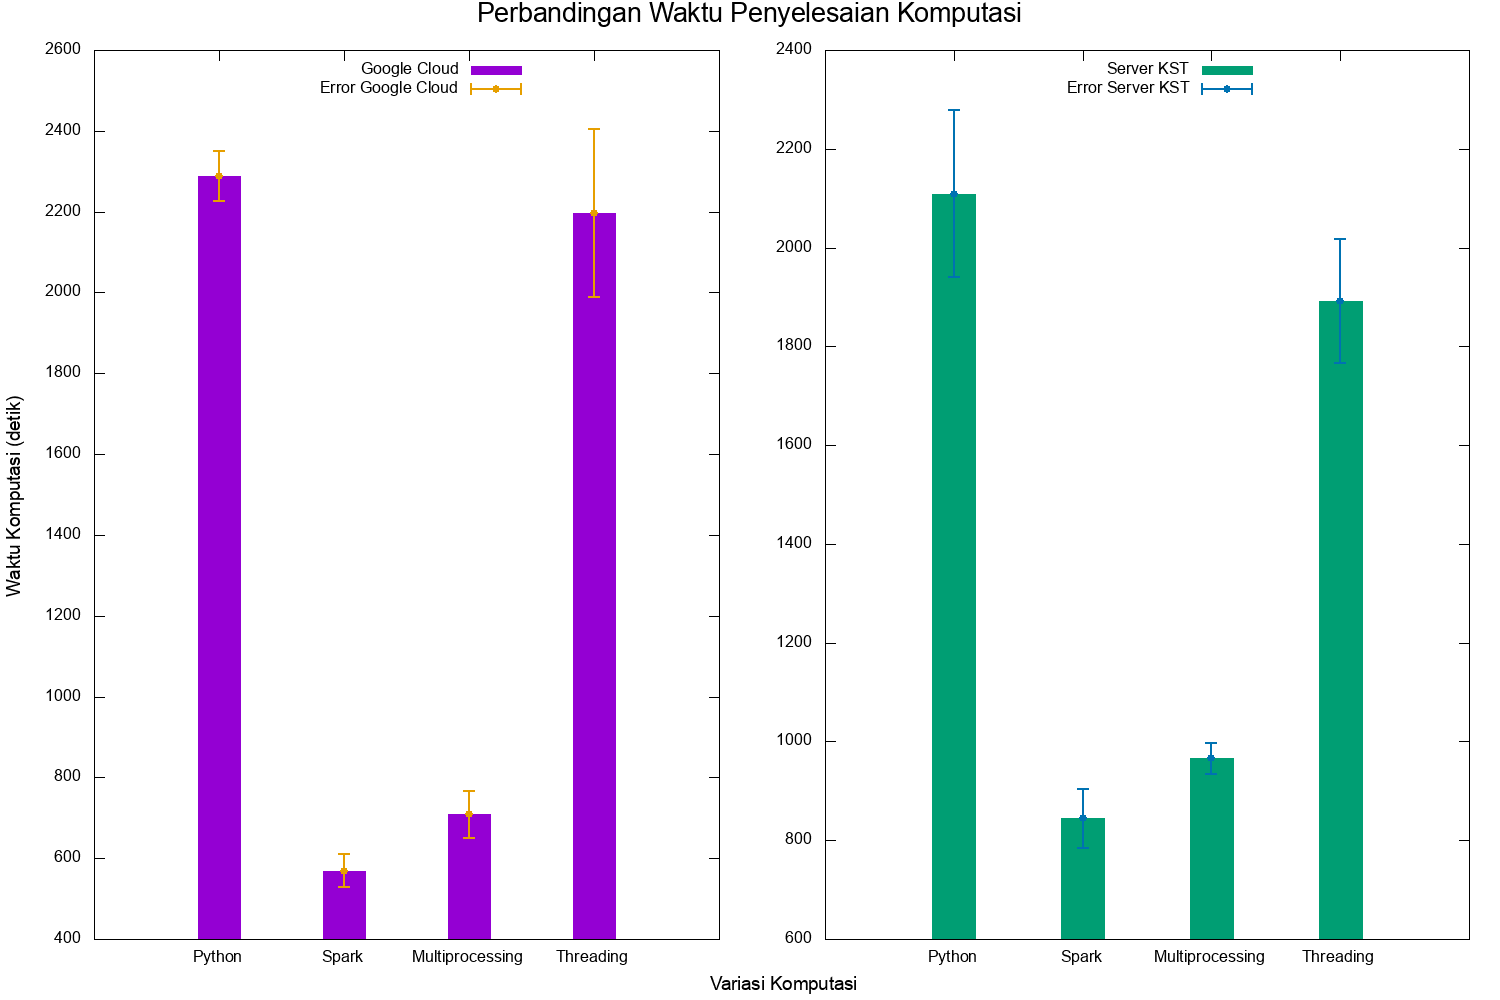
\includegraphics[width=12cm]{gambar/performa_komputasi.png}
	\captionof{figure}{Grafik Performa Komputasi}
	\label{performa_komputasi}
\end{center}

Dari Gambar \ref{performa_komputasi} terlihat bahwa menggunakan PySpark memiliki keunggulan dalam waktu komputasi. Waktu yang dibutuhkan untuk menghitung matriks berukuran $36*36$ hingga $4900*4900$ hanya sebesar $569,08$ detik untuk Server Google Cloud dan $844,72$ detik untuk Server KST. Pada urutan kedua tercepat yaitu menggunakan multiprocessing. Untuk multiprocessing dan PySpark memiliki cara kerja yang sama, yaitu menggunakan paralelisasi \textit{core} yang dimiliki oleh prosessor. Namun, untuk PySpark menggunakan paralelisasi kedalam jumlah pekerja (\textit{worker}) yang akan mengerjakan suatu tugas (\textit{task}) dengan \textit{In-Memory Processing}, yaitu proses yang akan dilakukan melibatkan \textit{memory}. Untuk \textit{load} dari server dapat dilihat di Lampiran 6 dan Lampiran 7. Kemudian jika dibandingkan antara penggunaan Server Google Cloud dengan Server KST, terdapat keunggulan untuk pemrosesan Python dan Threading untuk Server KST dan keunggulan untuk pemrosesan PySpark dan Multiprocessing untuk Server Google Cloud.

\subsection{Hasil Kalkulasi Absorbansi terhadap Perubahan Energi Eksitasi}

Hasil dari energi orbital kemudian dicari besar eksitasi dari HOMO ke LUMO tiap keadaannya. Untuk benzene, maka energi eksitasi tiap keadaan HOMO ke LUMO nya adalah,
\begin{table}[h]
	\centering
	\caption{Tabel Energi Eksitasi tiap Keadaan HOMO ke LUMO}
	\label{delE}
	\begin{tabular}{|c|c|} 
			\hline
			Eksitasi Orbital & $\Delta$E (eV) \\ \hline
			4 ke 3 & 3,16 \\ \hline
			4 ke 2 & 3,16 \\ \hline
			4 ke 1 & 4,74 \\ \hline
			5 ke 3 & 3,16 \\ \hline
			5 ke 2 & 3,16 \\ \hline
			5 ke 1 & 4,74 \\ \hline
			6 ke 3 & 4,74 \\ \hline
			6 ke 2 & 4,74 \\ \hline
			6 ke 1 & 6,32 \\ \hline
	\end{tabular}
\end{table}

Kemudian dari hasil vektor eigen, di masukkan kedalam persamaan \ref{lcao} untuk membuat persamaan \textit{linear combination atomic orbital} dan menjadi,
\begin{equation}
\begin{cases}
{\psi_1} = -0,408{\phi}_{1} - 0,577{\phi}_{2} + 0,408{\phi}_{3} - 0,577{\phi}_{4} - 0,031{\phi}_{5} + 0,045{\phi}_{6}\\
{\psi_2} = -0,408{\phi}_{1} - 0,289{\phi}_{2} - 0,408{\phi}_{3} + 0,289{\phi}_{4} - 0,515{\phi}_{5} - 0,520{\phi}_{6}\\
{\psi_3} = -0,408{\phi}_{1} + 0,289{\phi}_{2} + 0,408{\phi}_{3} + 0,289{\phi}_{4} - 0,484{\phi}_{5} + 0,477{\phi}_{6}\\
{\psi_4} = -0,408{\phi}_{1} - 0,289{\phi}_{2} - 0,408{\phi}_{3} + 0,289{\phi}_{4} + 0,484{\phi}_{5} + 0,477{\phi}_{6}\\
{\psi_5} = -0,408{\phi}_{1} + 0,289{\phi}_{2} + 0,408{\phi}_{3} + 0,289{\phi}_{4} + 0,515{\phi}_{5} - 0,521{\phi}_{6}\\
{\psi_6} = -0,408{\phi}_{1} + 0,577{\phi}_{2} - 0,408{\phi}_{3} - 0,577{\phi}_{4} + 0,031{\phi}_{5} + 0,045{\phi}_{6}
\end{cases}
\end{equation}

Konstanta fungsi gelombang inilah yang akan menginterpretasikan momen dipol yang dimiliki oleh Benzene. Untuk mencari momen dipol, dapat menggunakan rumus \ref{dipol}. Hasil yang didapatkannya adalah,
\begin{table}[h]
	\centering
	\caption{Tabel Momen Dipol Transisi}
	\label{momendipol}
	\begin{tabular}{|c|c|} 
		\hline
		Transisi Orbital & Momen Dipol Transisi (eV) \\ \hline
		4 ke 3 & 0,054 \\ \hline
		4 ke 2 & 1,249*$10^{-15}$ \\ \hline
		4 ke 1 & 7,772*$10^{-16}$ \\ \hline
		5 ke 3 & 1,804*$10^{-16}$ \\ \hline
		5 ke 2 & 1,284*$10^{-16}$ \\ \hline
		5 ke 1 & -8,327*$10^{-17}$ \\ \hline
		6 ke 3 & -2,689*$10^{-16}$ \\ \hline
		6 ke 2 & -4,996*$10^{-16}$ \\ \hline
		6 ke 1 & -1.183*$10^{-15}$ \\ \hline
	\end{tabular}
\end{table}

Momen dipol transisi terbesar adalah saat transisi orbital 4 ke 3. Hal ini disebabkan karena transisi tersebut terletak pada titik terluar yang menyebabkan transisinya akan membutuhkan energi yang besar, dan transisi orbital 4 ke 3 merupakan transisi yang terjadi pada celah energi dari senyawa tersebut.

Dari hasil perubahan energi eksitasi tiap orbital (Tabel \ref{delE}) dan hasil momen dipol transisi (Tabel \ref{momendipol}) akan dihitung besar absorbansi terhadap perubahan energi eksitasi tiap orbital menggunakan persamaan \ref{absorbansi}. Jika diplot, grafik absorpsi terhadap $\Delta$E nya menjadi, 
\begin{center}
	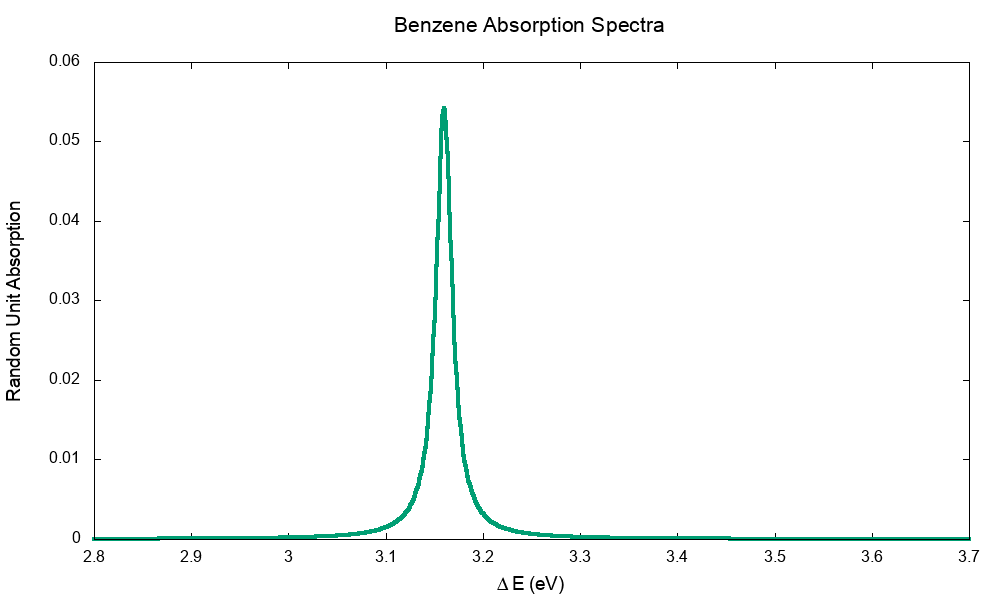
\includegraphics[width=10cm]{gambar/spectra-benzene.png}
	\captionof{figure}{Spektrum Absorbansi terhadap Perubahan Energi Eksitasi pada Benzene}
	\label{absorbance_benzene}
\end{center}

Dari gambar \ref{absorbance_benzene}, terlihat bahwa titik puncak penyerapan energi terjadi pada $\Delta$E sebesar $\pm$ 3.15 eV dan ini adalah besar celah energi yang dimiliki oleh Benzene. Hal ini disebabkan karena titik absorbsi energi menggambarkan besar energi yang akan diserap oleh elektron, dan energi yang diserap akan membuat elektron tereksitasi ke keadaan dengan energi yang lebih besar.

Apabila jumlah atom karbon diperbanyak, maka puncak absorbansi yang terjadi akan bergeser ke kiri (mendekati $\Delta$E = 0). Terlihat pada Gambar \ref{absorbance_graphene50} dan Gambar \ref{absorbance_graphene400}.
\begin{center}
	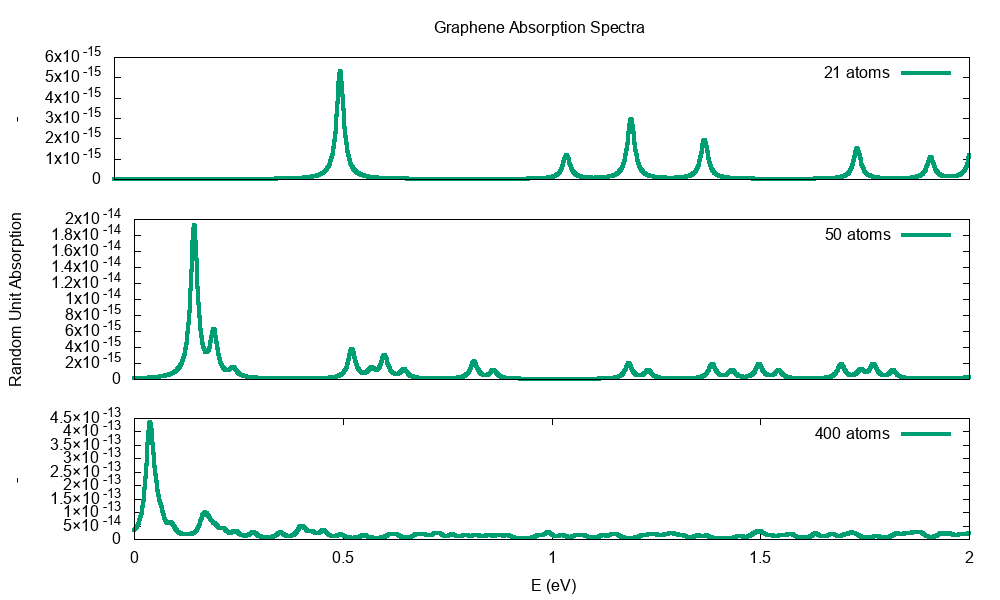
\includegraphics[width=12cm]{gambar/spectra-graphene.png}
	\captionof{figure}{Spektrum Absorbansi terhadap Perubahan Energi Eksitasi pada Graphene}
	\label{absorbance_graphene50}
\end{center}

Selain itu, terdapat puncak-puncak kecil yang menunjukkan masih ada energi yang terserap oleh elektron. Ini menunjukkan bahwa Graphene bersifat metalik yaitu sebagai konduktor yang baik akibat perpindahan atau eksitasi elektron yang terjadi sangatlah mudah.


\chapter*{BAB V \\ KESIMPULAN DAN SARAN}
\addcontentsline{toc}{chapter}{BAB V KESIMPULAN DAN SARAN}
\setcounter{chapter}{5}
\setcounter{section}{0}
\setcounter{figure}{0}
\thispagestyle{myplain}
\section{Kesimpulan}
	Telah dirancang algoritma untuk membangun matriks Hamiltonian dan kalkulasi spektrum absorbsi menggunakan bahasa pemrograman Python. Data-data yang akan didapatkan meliputi: celah energi (\textit{gap energy}), energi eksitasi tiap tingkat orbital molekul ($\Delta$E), momen dipol transisi, dan absorbsi. Celah energi yang didapatkan akan mengecil jika semakin banyak atom karbon yang dimiliki oleh Graphene. Ini disebabkan karena saat atom karbon bertambah, jarak energi antar orbital molekulnya akan semakin kecil atau \textit{Density of States} nya bertambah padat dan menyebabkan elektron lebih mudah untuk bereksitasi. Akurasi yang didapatkan dari hasil perhitungan celah energi yaitu: celah energi Benzene pada literatur sebesar 3.1 eV \cite{Masiak2017} dan hasil komputasi sebesar 3.1599 eV dengan kesalahan relatif sebesar 18,95\%. Untuk akurasi Graphene 3.5 nm, didapatkan hasil literatur sebesar 0.4 eV dan hasil komputasi sebesar 0.5219 eV dengan kesalahan relatif sebesar 32,275\%. Hal ini diakibatkan Teori Hückel merupakan persamaan semi-empirik dan hanya melibatkan interaksi tetangga terdekatnya saja. Dalam penghitungan besar energi orbital molekul, dilakukan dengan menggunakan variasi komputasi Python, \textit{PySpark}, \textit{Multiprocessing} dan \textit{Threading}. Dari keempat variasi tersebut, PySpark memiliki keunggulan dalam waktu komputasi yang dibutuhkan dengan rata-rata $569,08$ detik untuk Server Google Cloud dan $844,72$ detik untuk Server KST. Setelah menghitung celah energi, lalu dicari energi eksitasi tiap tingkat orbital dan momen dipol transisinya dan akan didapatkan besar absorbansi tiap perubahan energi eksitasi. Jika di plot kedalam grafik, akan terlihat puncak absorbsi yang akan menginterpretasikan besar celah energi yang dimiliki oleh Graphene. Hal ini karena momen dipol transisi akan menggambarkan besar energi transisi orbital molekulnya, dan energi transisi tertinggi akan menggambarkan transisi dari keadaan HOMO ke LUMO yang merupakan celah energi. Puncak absorbansi akan semakin menggeser mendekati $\Delta E = 0$ saat atom karbon nya bertambah dan juga terdapat puncak-puncak kecil dari absorbansi yang menunjukkan Graphene merupakan bahan dengan sifat metalik dan konduktor yang baik.
\section{Saran}
	Dari penelitian yang sudah dilakukan, terdapat beberapa masukan untuk penelitian selanjutnya yaitu:
	\begin{enumerate}
		\item Membuat plot spektrum absorbansi terhadap panjang gelombang dalam nanometer untuk melihat besar penyerapan energi di setiap panjang gelombangnya sesuai kerja UV-Vis Spektrometer
		\item Membuat kode untuk mengkalkulasi spektrum absorbsi Graphene Oxide dan Reduced Graphene Oxide
		\item Menganimasikan perilaku orbital molekul pada Graphene untuk mempermudah pembaca dalam memahami peristiwa tersebut
		\item Melihat pengaruh \textit{Meta-Stable Energy} yang menyebabkan terdapat energi yang tersisa pada grafik absorbsi
		\item Menggunakan performa Apache Spark dengan \textit{full-power} agar performa komputasi yang dihasilkan lebih baik
	\end{enumerate}
\addcontentsline{toc}{chapter}{DAFTAR PUSTAKA}
\printbibliography[title = {DAFTAR PUSTAKA}]
\chapter*{\centering DAFTAR LAMPIRAN }
\thispagestyle{myplain}
\section*{Lampiran 1: Kode Kalkulasi Huckel dan Absorbansi}
\addcontentsline{toc}{chapter}{DAFTAR LAMPIRAN}
\addcontentsline{toc}{section}{Lampiran 1: Kode Kalkulasi Huckel dan Absorbansi}
\lstinputlisting[language=Python]{koding/huckel.py}

\section*{Lampiran 2: Kode Eksekusi dengan Python}
\addcontentsline{toc}{section}{Lampiran 2: Kode Eksekusi dengan Python}
\lstinputlisting[language=Python]{koding/main.py}

\section*{Lampiran 3: Kode Eksekusi dengan PySpark}
\addcontentsline{toc}{section}{Lampiran 3: Kode Eksekusi dengan PySpark}
\lstinputlisting[language=Python]{koding/main_spark.py}

\section*{Lampiran 4: Kode Eksekusi dengan Multiprocessing}
\addcontentsline{toc}{section}{Lampiran 4: Kode Eksekusi dengan Multiprocessing}
\lstinputlisting[language=Python]{koding/main_mp_pool.py}

\section*{Lampiran 5: Kode Eksekusi dengan Threading}
\addcontentsline{toc}{section}{Lampiran 5: Kode Eksekusi dengan Threading}
\lstinputlisting[language=Python]{koding/main_thread.py}

\section*{Lampiran 6: \textit{Process Load} dengan Multiprocessing}
\addcontentsline{toc}{section}{Lampiran : \textit{Process Load} dengan Multiprocessing}
\begin{center}
	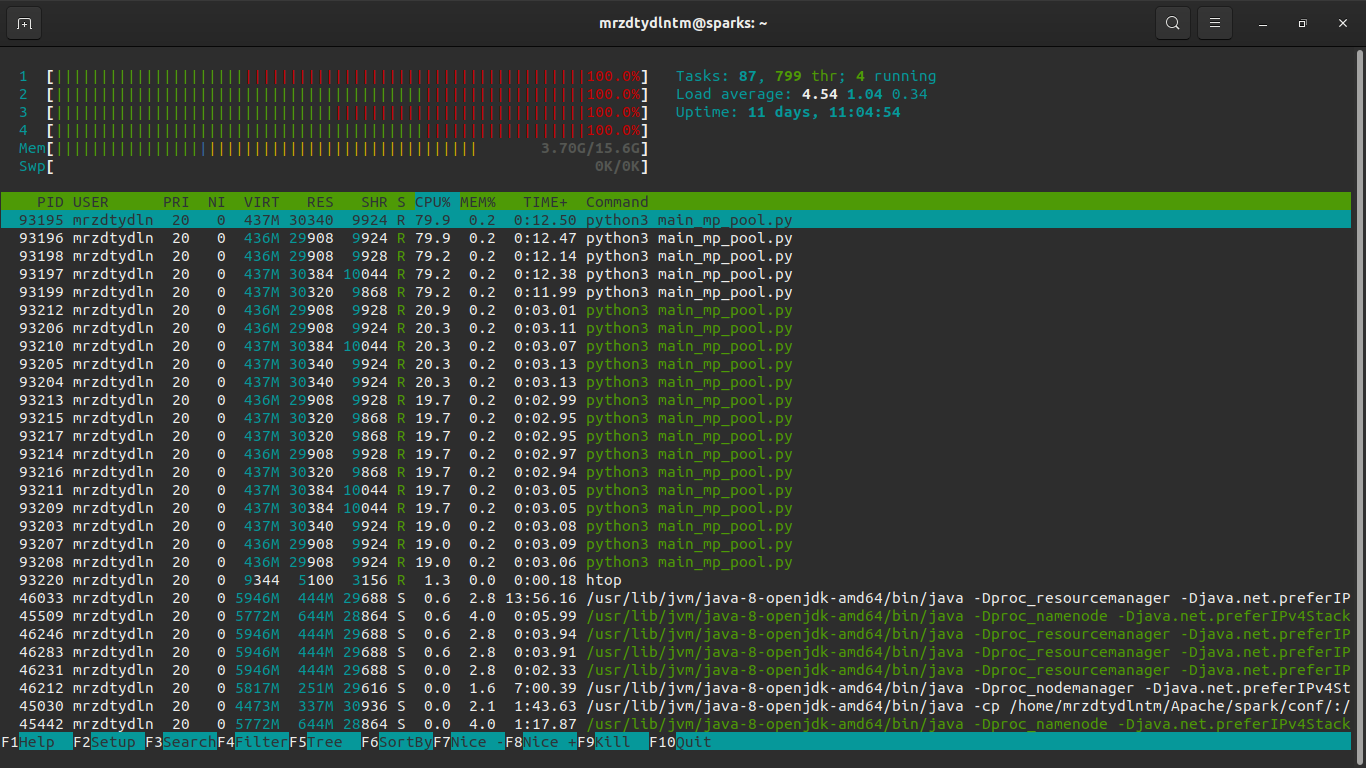
\includegraphics[width=12cm]{gambar/mp_pool.png}
\end{center}

\section*{Lampiran 7: \textit{Process Load} dengan PySpark}
\addcontentsline{toc}{section}{Lampiran : \textit{Process Load} dengan PySpark}
\begin{center}
	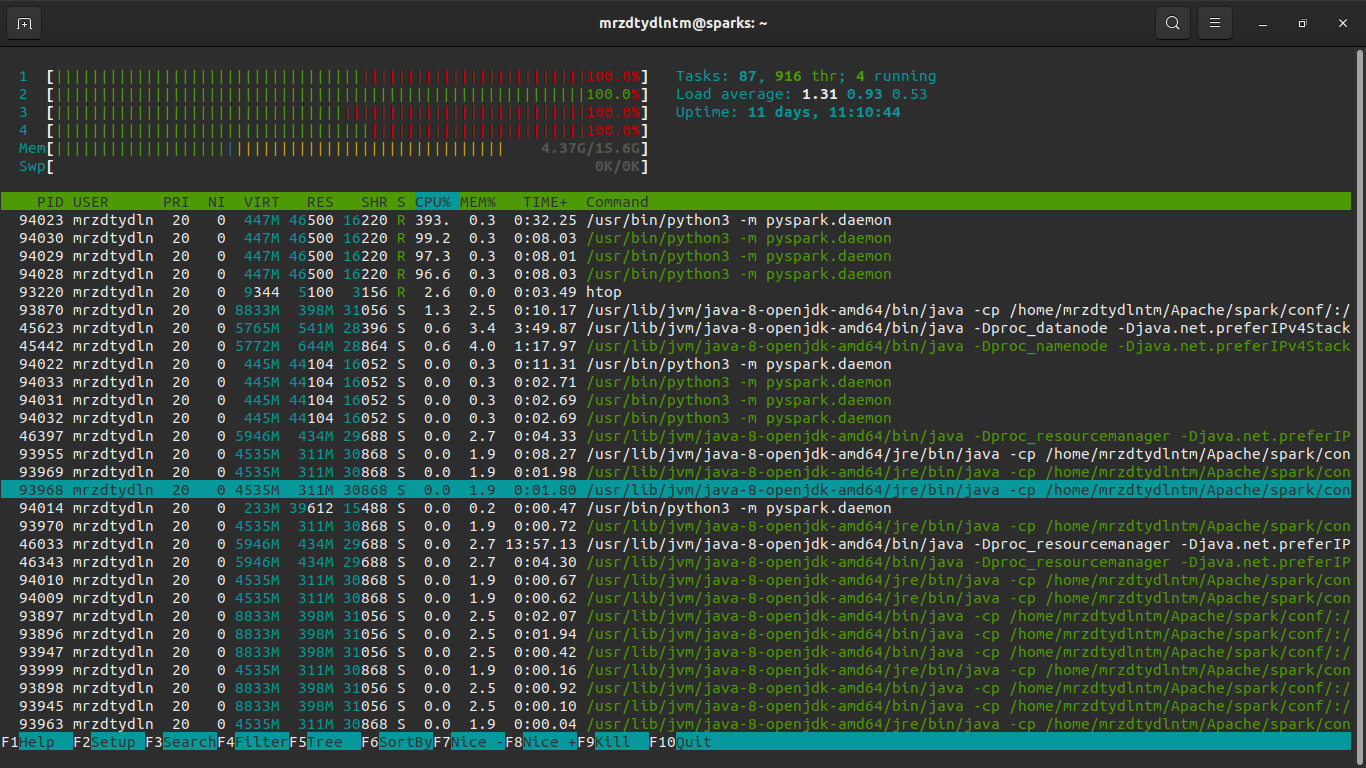
\includegraphics[width=12cm]{gambar/spark-submit.png}
\end{center}

\section*{Lampiran 8: Spark Master pada Server Google Cloud}
\addcontentsline{toc}{section}{Lampiran 8: Spark Master pada Server Google Cloud}
\begin{center}
	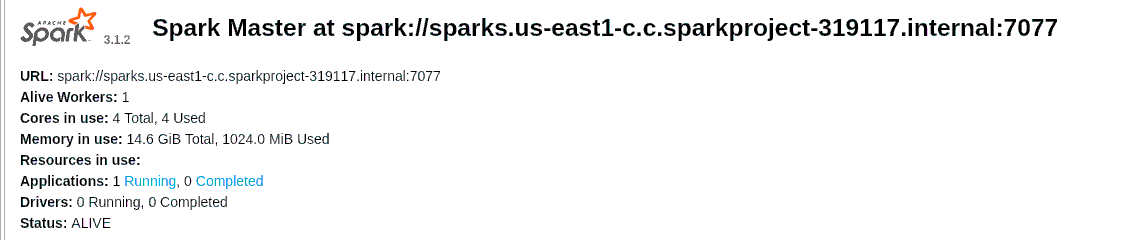
\includegraphics[width=13cm]{gambar/gcp.png}
\end{center}

\section*{Lampiran 9: Spark Master pada Server KST}
\addcontentsline{toc}{section}{Lampiran 8: Spark Master pada Server KST}
\begin{center}
	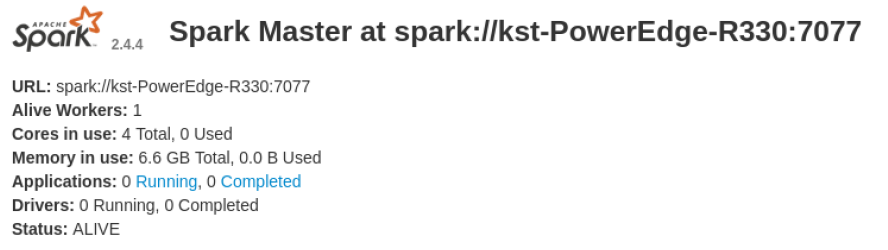
\includegraphics[width=11cm]{gambar/kst.png}
\end{center}

\section*{Lampiran 10: Spesifikasi Server Google Cloud}
\addcontentsline{toc}{section}{Lampiran 10: Spesifikasi Server Google Cloud}
\begin{center}
	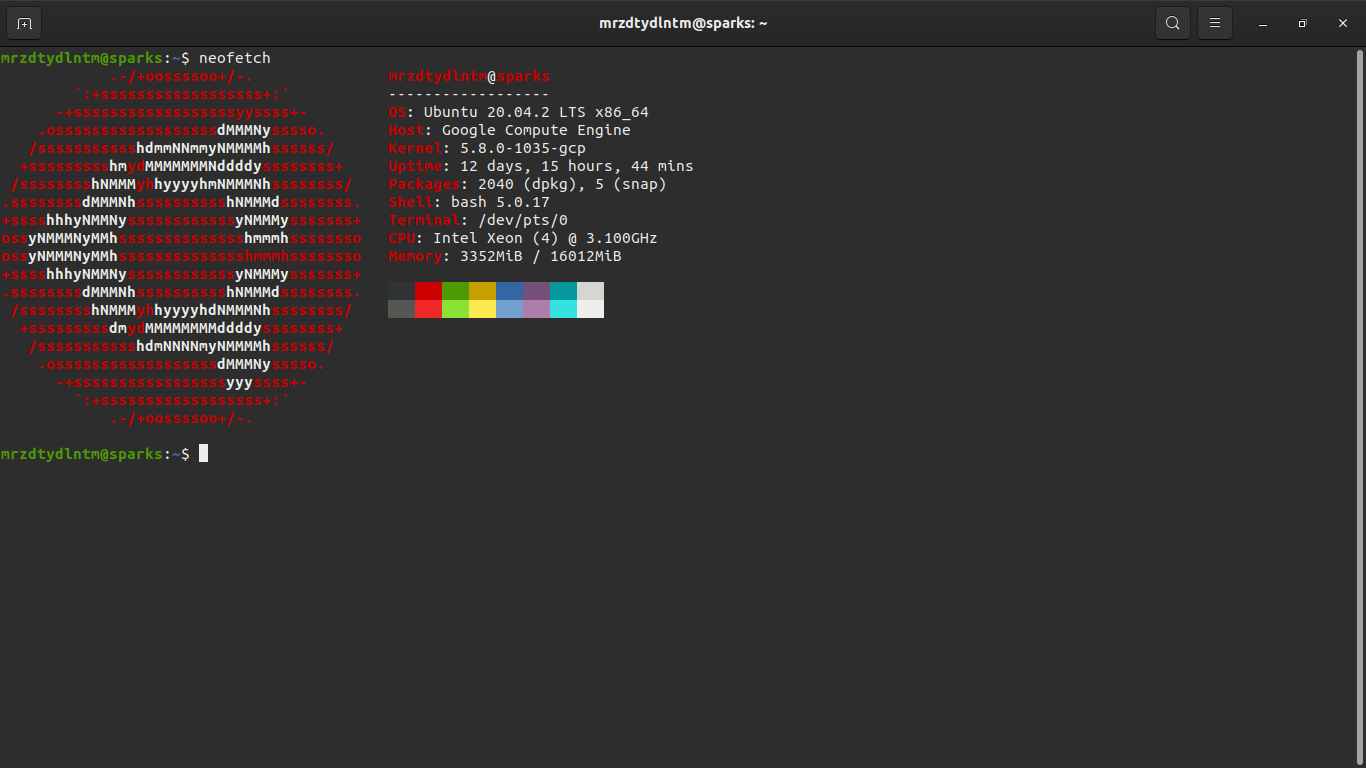
\includegraphics[width=12cm]{gambar/neofetch-gcp.png}
\end{center}

\end{document}
